\chapter{Experimentos y resultados}\label{chapter5}

% **************************** Define Graphics Path **************************
\graphicspath{{Chapter5/Figs/}}


En este capítulo se describe la experimentación y lo resultados obtenidos
que muestran la mejora en el desempeño de un agente que aprende
con y sin información adicional de un grafo causal.
Para probar el concepto propuesto se atacan dos problemas: la tarea de clásica del taxi \cite{Dietterich:2000:HRL:1622262.1622268} y la de los
interruptores de luz, descrita en el Capítulo \ref{chapter4}.
En resumen, los experimentos consisten en integrar el grafo $\mathcal{D}$ a la política $\epsilon$ greedy
en el algoritmo $Q$-learning \cite{watkins1992q}.
En la política $\epsilon$-greedy en vez de mantener fijo a $\epsilon$, se propone empezar motivando al agente a explorar y usar
el modelo causal e ir disminuyendo $\epsilon$ para dar más peso a la explotación.
Se comparan cuatro algoritmos, \textit{Q-learning sin información
adicional}, \textit{Q-learning con una estructural causal completa}, \textit{Q-learning con una estructura parcial} y un \textit{Q-learning con una estructura incorrecta}.
Cada uno de los algoritmos se ejecuta en una versión determinista y 
otra estocástica del ambiente. 
En las siguientes secciones se describen a detalle los experimentos realizados y los resultados. Todo el software desarrollado está 
disponible en \url{https://github.com/ivanfeliciano/causal_rl/}.


\section{Problema del taxi}

\subsection{Descripción de la tarea}

El primer problema a resolver es la tarea clásica del taxi \cite{Dietterich:2000:HRL:1622262.1622268}.
La Figura \ref{fig:taxi} muestra gráficamente el problema.
Existen cuatro posiciones en el mundo marcadas como R, B, G, y Y. 
La tarea es episódica. En cada episodio, 
el taxi comienza en un cuadro aleatoriamente elegido. 
Existe un pasajero en una de la cuatro posiciones (también elegida
aleatoriamente), y el pasajero desea ser transportado a una de las
cuatro zonas.
El taxi debe dirigirse a la posición del pasajero, recogerlo, ir a su destino y dejarlo.
El episodio termina cuando el pasajero es dejado en su destino.

\begin{figure}[H]
    \centering
    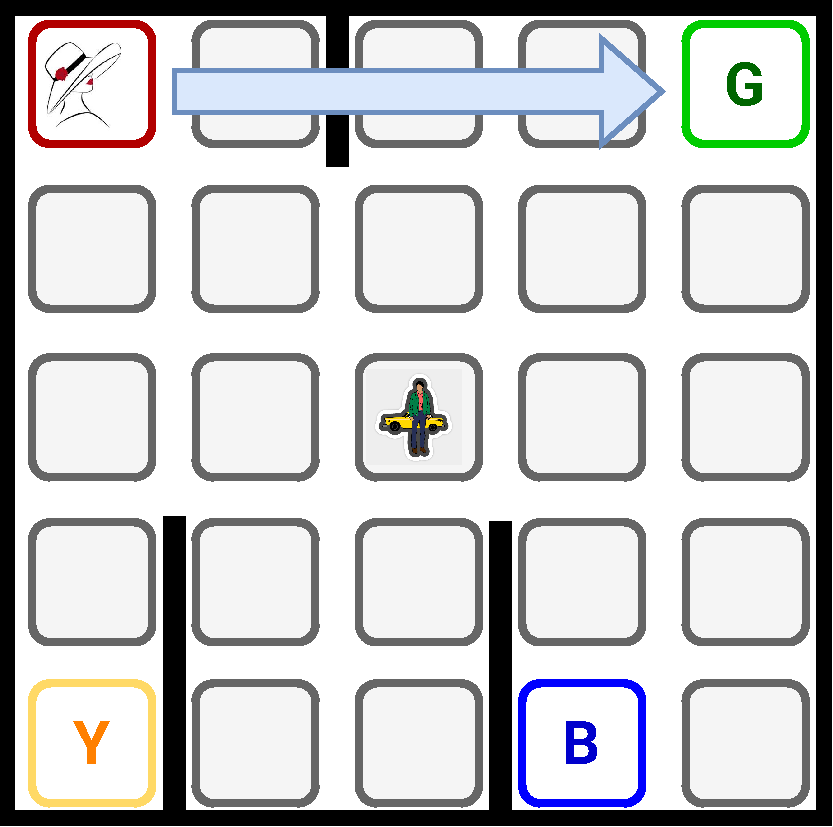
\includegraphics[scale=0.25]{Chapter5/Figs/taxi-env.pdf}
    \caption{La cuadrícula del ambiente del taxi. El taxi se encuentra en el cuadro central. En esta configuración del mundo, el objetivo es recoger al pasajero en la posición R y llevarlo a la posición G.}
    \label{fig:taxi}
\end{figure}

El conjunto de acciones $\mathcal{A}$ está compuesto por seis elementos: una acción para recoger $a_1$, una para dejar $a_2$ y
cuatro acciones de 
navegación que trasladan al taxi un cuadro al norte, sur, 
este u oeste, denotadas por $a_3, \dots, a_6$, respectivamente.
Existe una recompensa de -1 por cada acción, una recompensa adicional de 20 por cada pasajero llevado a su destino 
exitosamente y una penalización de -10 por acciones ilegales
de recolección y dejado.
El espacio de estados $\mathcal{S}$ tiene como elementos 
500 tuplas de tres elementos donde describen los 25 cuadros, las 5 posiciones del pasajero (incluyendo cuando está en el taxi) y los 4 destinos.


% Aquí ahondar más sobre el conjunto X y G, quienes lo compoenen y como está de pequeñito el problema
El conjunto $\mathcal{X}$ contiene 4 variables que traducen las tuplas con las posiciones del taxi y del pasajero en variables binarias. $x_1$
es la variable que dice si el taxi está en la misma posición que el
pasajero, $x_2$ es la variable que denota si el pasajero es llevado dentro del taxi, $x_3$ describe si el taxi está en la posición destino,
y $x_4$ es la variable que representa al estado de que el pasajero es entregado correctamente. Es una tarea relativamente simple y $x_1 \neq x_3$, por lo tanto las metas son $\mathcal{G} = \{\mathbf{g_1}, \mathbf{g_2}\}$, donde $\mathbf{g_1} = [1, 1, 0 , 0]$ y $\mathbf{g_2} = [0,1,1,1]$. El primer vector se puede ver como el sub objetivo de 
llevar subir al pasajero al taxi y el segundo vector es la meta general, 
entregar al pasajero en su destino.
El grafo causal $\mathcal{D}$ entre las variables de acción y los estados se puede 
ver en la Figura \ref{fig:cm-taxi}. Para este problema, los efectos
necesitan de todas sus causas para suceder, por ejemplo, para que el
pasajero esté dentro del taxi, $x_2 = 1$, entonces se debe actuar
subiéndolo al vehículo $a_1$ y además estar en la misma ubicación que
el pasajero.

\begin{figure}[H]
    \centering
    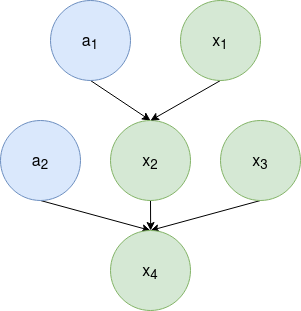
\includegraphics[scale=0.3]{Chapter5/Figs/causal_structure_taxi.png}
    \caption{Propuesta de una estructura causal para la tarea del taxi.}
    \label{fig:cm-taxi}
\end{figure}


\subsection{Configuración experimental}

Debido a la poca información que ofrece el grafo $\mathcal{D}$ y al tamaño de $\mathcal{G}$, para este problema no se ahonda en realizar experimentos con diferentes configuraciones. Por lo
tanto, sólo se comparan dos algoritmos,
el algoritmo Q-learning con y sin la estructura causal.
Además, los dos algoritmos se prueban sobre dos versiones del ambiente, una determinista
y otra estocástica. Los valores de los parámetros para los experimentos se muestran en el Cuadro \ref{tab:tax-params}. Se ejecutan $M$ experimentos y cada experimento consiste de ejecutar cada algoritmo $k$ de episodios. La medida
de desempeño es la recompensa promedio por episodio. El valor de $\epsilon$ se va decrementando en cada paso de tiempo de entrenamiento $t$ de forma lineal ($\epsilon = \max(\epsilon_{\min}, mt + \epsilon_{\max})$, $m < 0$ y representa la tasa de decremento)
con respecto al
número de episodios, por lo que se fomenta la exploración y el uso del modelo causal al principio y posteriormente se explota la información de $Q$.

\begin{table}[H]
\centering
\caption{Parámetros para las versiones del algoritmo Q-learning.}
\label{tab:tax-params}
\begin{tabular}{ll}
\hline
Parámetro                                                                                      & Valor    \\ \hline
$\alpha$                                                                                       & 0.8      \\
$\gamma$                                                                                       & 0.95     \\
$\epsilon_{\min}$                                                                              & 0.1      \\
$\epsilon_{\max}$                                                                              & 1.0      \\
$m$                                                                                            & -0.0045 \\
$k$                                                                                            & 5000     \\
$M$                                                                                            & 10       \\
\begin{tabular}[c]{@{}l@{}}Probabilidad de\\ transición en ambiente\\ estocástico\end{tabular} & 0.7      \\ \hline
\end{tabular}
\end{table}

\subsection{Resultados}

En la Figura \ref{fig:results-taxi} se muestran los resultados obtenidos
para ambas configuraciones del ambiente (determinista y estocástico) donde
los valores de los parámetros se describen en el Cuadro \ref{tab:tax-params}.
La recompensa promedio por episodio para el método propuesto y para el algoritmo
original Q-learning están en color naranja y azul, respectivamente. 
Los resultados muestran que el algoritmo Q-learning guiado por el grafo da un salto inicial alto y mantiene una recompensa promedio mucho mayor que la versión sin información adicional. Esto era esperado, ya que 
no inicia una exploración a ciegas. Por otra parte, para el caso 
del ambiente estocástico, parecen comportarse de manera similar después de los
primeros 1000 episodios. Esto se puede deber a que tal vez la información del 
grafo no ayuda los suficiente, ya que a pesar de que tal vez existen
conexiones entre acciones y estados que no se están tomando en cuenta.


\begin{figure}[H]
  \centering
  \subfloat[Ambiente determinista.]{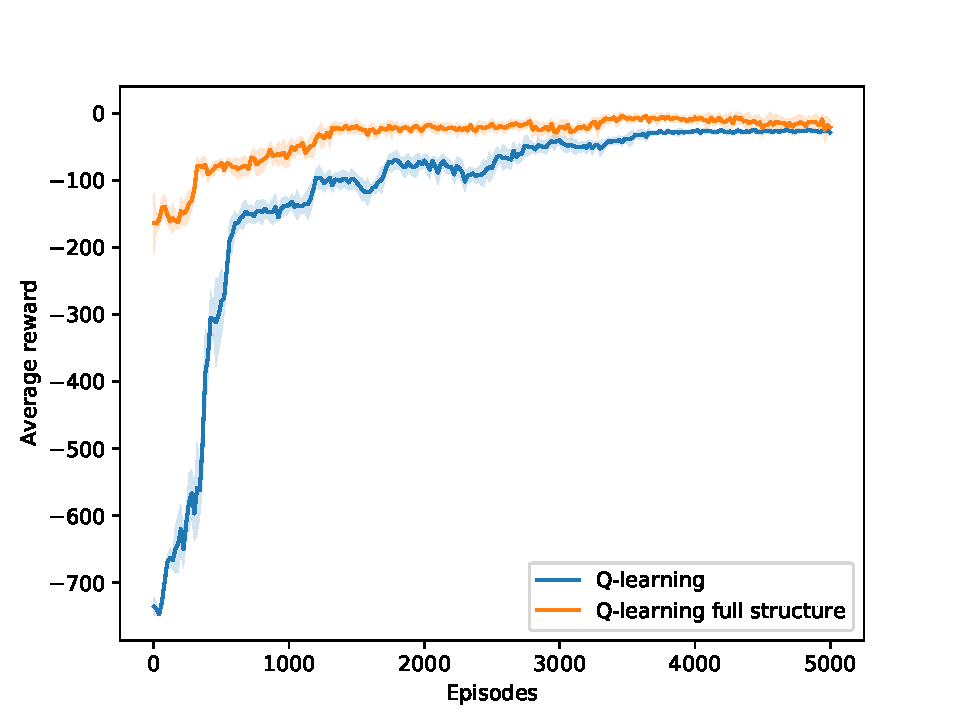
\includegraphics[width=0.5\textwidth]{Chapter5/Figs/taxiDet500010.pdf}\label{fig:taxi-rew-det}}
  \hfill
  \subfloat[Ambiente estocástico.]{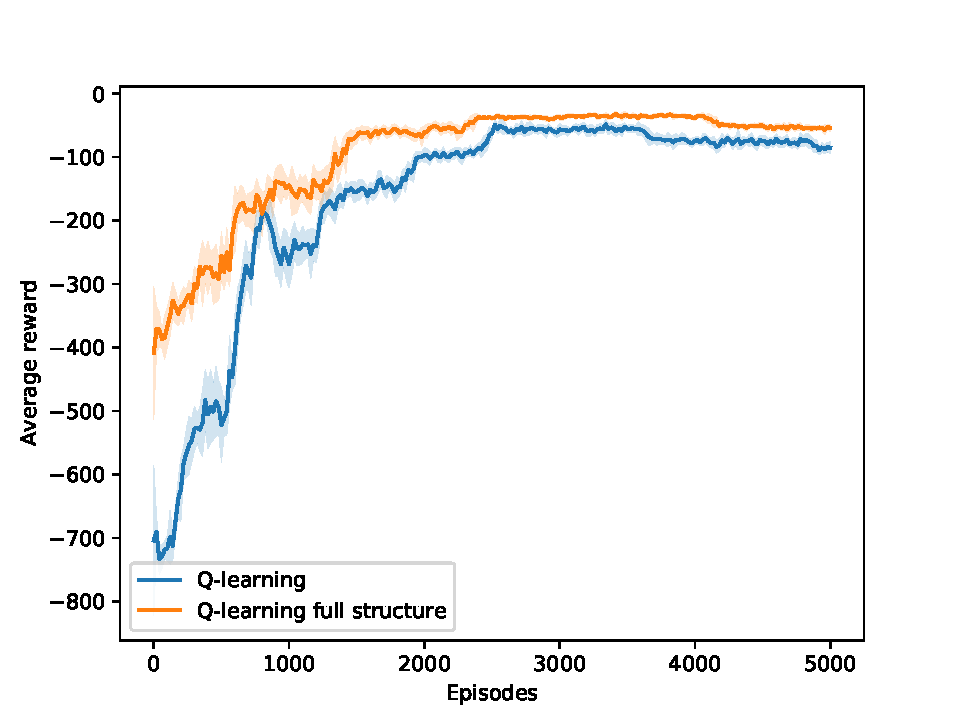
\includegraphics[width=0.5\textwidth]{Chapter5/Figs/taxiSto500010.pdf}\label{fig:taxi-rew-sto}}
  \caption{Comparación del desempeño para los dos algoritmos en 5000 episodios. La región sombreada es la desviación estándar para 10 experimentos.}
  \label{fig:results-taxi}
\end{figure}
\section{Problema de los interruptores de luz}

\subsection{Descripción de la tarea}
Para los experimentos de esta sección se ataca la tarea de control de interruptores de luz propuesta en \cite{nair2019causal} y descrita de manera general en la Sección \ref{section:switches-example}. Un agente tiene el control
de $N$ interruptores que controlan $N$ luces en un sitio.
Cada acción $a\in \mathcal{A}$ corresponde a mover un interruptor o 
a no mover ninguno, por lo tanto $|\mathcal{A}| = N + 1$.
El agente puede percibir dos tipos de señales del ambiente,
una imagen $s$ con una vista cenital del sitio, o vectores binarios $x \in \{0,1\}^N$ de 
macro-variables que codifican las luces prendidas, donde
$x_i = 1$ si la luz en la zona $i$ está prendida, de otro modo 
toma el valor $x_i = 0$.

Se exploran tres tipos de estructuras causales entre los
interruptores y las luces: \textit{uno-a-uno},
\textit{causa común} y \textit{efecto común}.
En los problemas con estructuras uno-a-uno cada interruptor corresponde a una sola luz.
Para el segundo tipo, de causa común, todas
las luces son controladas a lo más por un interruptor pero un
solo interruptor puede controlar más de una luz.
El tercer caso son estructuras de efecto común, donde cada interruptor
controla una sola luz, aunque múltiples interruptores
pueden controlar la misma luz. De manera visual, los tres tipos de estructuras
se muestran en la Figura \ref{fig:struct}.

\begin{figure}[H]
    \centering
    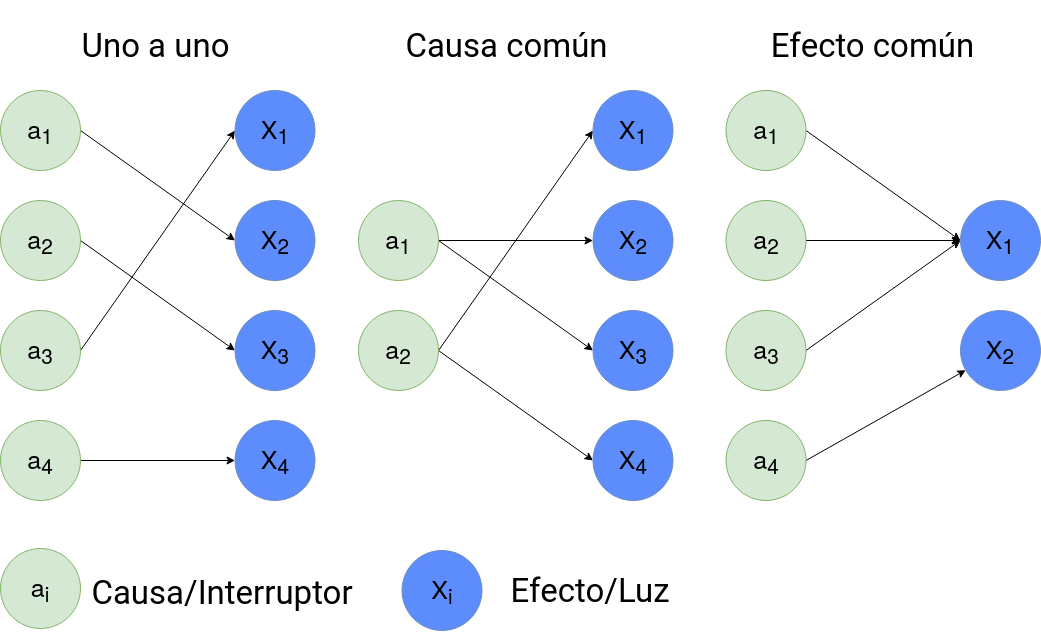
\includegraphics[scale=0.3]{Chapter5/Figs/switches_struct.png}
    \caption{Tipos de estructuras causales subyacentes posibles.}
    \label{fig:struct}
\end{figure}
La recompensa inmediata $r$ brindada al agente se calcula obteniendo la distancia entre el vector de variables de estado alto nivel $\mathbf{x}$ y el vector meta $\mathbf{g}$. En este problema se usa la distancia euclidiana.


\subsection{Configuración experimental general}

En las siguientes secciones se compara el desempeño 
del método propuesto en diferentes escenarios, principalmente, para mostrar 
las posibilidades y ventajas de usar un información del grafo causal, completa, incompleta e incluso incorrecta. 
% A pesar de ser diferentes
% experimentos, éstos comparten la configuración de algunos elementos, por ejemplo, 
% la medida de desempeño, el número de variables $N$, etc.
Se comparan cuatro algoritmos, teniendo como base
el método Q-learning. Donde la diferencia subyace en la cantidad y calidad de la información adicional con la que cuenta. A continuación, se describen de manera breve los métodos
comparados.

\begin{itemize}
    \item \textit{Q-learning sin información adicional}. Este método sirve como
    línea de base para medir que tanto mejora el aprendizaje. El algoritmo, dependiendo del espacio de estados sobre el que se trabaje, es el 
    método básico de Q-learning \cite{watkins1992q} o Q-learning profundo \cite{mnih2013playing}, para estados
    discretos y continuos, respectivamente. La selección de acciones se lleva a cabo mediante una política $\epsilon$ greedy clásica.
    \item \textit{Q-learning + estructura causal completa}. Durante la política de selección de acciones, el agente cuenta con la estructura causal del ambiente completa y verdadera $\mathcal{D}$.
    \item \textit{Q-learning + estructura causal incompleta}. En este caso, el agente cuenta con un subgrafo $\mathcal{D'}$ del grafo $\mathcal{D}$. Este subgrafo se genera eliminando aristas de $\mathcal{D}$ aleatoriamente.
    \item \textit{Q-learning + estructura causal incorrecta}. Este algoritmo consulta un modelo $\mathcal{D}''$ con relaciones espurias y sin algunas relaciones verdaderas. Este grafo $\mathcal{D}''$ se obtiene generando un subgrafo de $\mathcal{D}$ como en el caso anterior y agregando aristas aleatoriamente.
\end{itemize}

\begin{figure}
  \centering
  \subfloat[$\mathcal{D}$.]{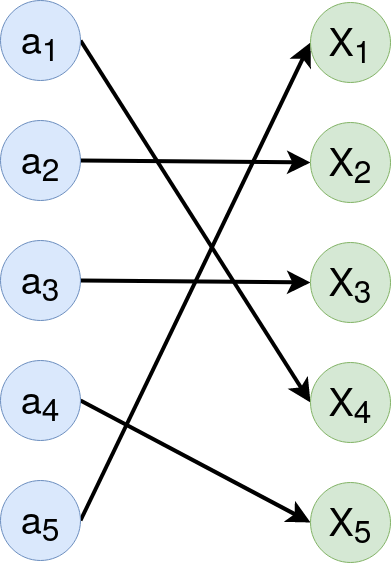
\includegraphics[width=0.2\textwidth]{Chapter5/Figs/completeD.png}\label{fig:completeD}}
  \qquad
  \subfloat[$\mathcal{D}'$]{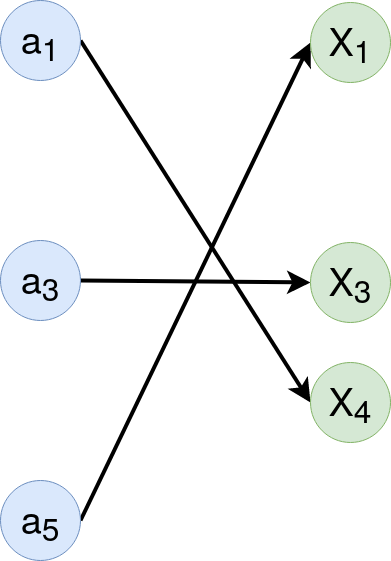
\includegraphics[width=0.2\textwidth]{Chapter5/Figs/incompleteD.png}\label{fig:incompleteD}}
%   \hfill
    \qquad
  \subfloat[$\mathcal{D}''$]{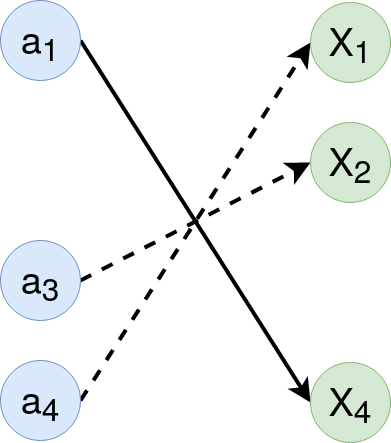
\includegraphics[width=0.2\textwidth]{Chapter5/Figs/wrongD.png}\label{fig:wrongD}}
  \caption{Ejemplo de los tres tipos de información con los que puede  contar el algoritmo Q-learning. El tipo de estructura
  del problema es uno-a-uno. Las aristas dirigidas punteadas describen conexiones espurias.}
  \label{fig:types-info-dag}
\end{figure}

Para medir el desempeño de los algoritmos se evalúa la recompensa
promedio sobre una serie de experimentos.
Cada experimento consiste en ejecutar el algoritmo de aprendizaje durante $k$ episodios, en 
un ambiente con una estructura causal fija $\mathcal{D}$ y donde se busca alcanzar la meta $\mathbf{g}$.
La recompensa promedio para el $i$ ésimo episodio está dada por
$R^{i} = \frac{1}{H}\sum_{t=0}^H r(\mathbf{x}_t, \mathbf{g})$,
donde $H$ corresponde al tamaño del episodio.
El vector $\mathbf{R_i}$, del $i$ ésimo experimento contiene las recompensas promedio por cada episodio, y se define como
$\mathbf{R_i} = (R^{1}, \dots, R^k)$.

Finalmente, la medida de comparación entre algoritmos es
el promedio de los vectores $\mathbf{R_i}$, $i\in [1, M]$,  obtenidos en $M$ experimentos. Esta medida, denotada como  $average$ puede escribirse como 
\begin{equation}
\label{eq:average}
average(\mathbf{R_1}, \dots, \mathbf{R_M}) = \frac{1}{M}(\sum^M_i \mathbf{R_{i}^1}, \dots, \sum^M_i\mathbf{R_{i}^k}),    
\end{equation}

donde $M$ es el número de experimentos y el $\mathbf{R_i^j}$ indica la recompensa promedio obtenida en el $j$ ésimo episodio del $i$ ésimo experimento.

El parámetro $\epsilon$ se disminuye linealmente, donde
en cada selección de acción va decreciendo hasta llegar
un valor mínimo. La regla de actualización de $\epsilon$ en
el paso de tiempo $t$ se puede definir como $\epsilon = \max(\epsilon_{\min}, (\epsilon_{\min} - \epsilon_{\max}) \times t/ (N \times k \times \delta) + \epsilon_{\max})$. Donde $0 < \delta \leq 1$, es un factor para controlar
que tan rápido se alcanza el valor de $\epsilon$  mínimo, entre más cercano a 0,
termina más rápido la exploración.
% Con excepción
% del Experimento 2 (Sección \ref{subsection:exp-epsilon}), donde se cambia el denominador de la
% tasa de decremento para que éste se más rápido.

%Los experimentos se llevan a cabo en dos versiones del ambiente, una discreta y otra estocástica. 
Son tres los experimentos que se realizan. El primer experimento tiene 
como objetivo mostrar el comportamiento de modificar a
diferentes porcentajes la estructura causal $\mathcal{D}$ para obtener $\mathcal{D'}$ y $\mathcal{D}''$. El segundo experimento es con respecto a cambiar la tasa de decremento
de $\epsilon$ para llegar más rápido o lento a explotar 
más constantemente. El tercer experimento, es probar
el algoritmo cuando no se tienen las variables
de alto nivel como observaciones directas, por lo tanto,
se trabaja sobre un espacio de estados continuo. En general,
algunos de los parámetros que se comparten entre los experimentos se muestran en el Cuadro \ref{tab:switch-params}.

\begin{table}[H]
\centering
\caption{Valores para algunos parámetros de los algoritmos.}
\label{tab:switch-params}
\begin{tabular}{ll}
\hline
Parámetro                                                                                      & Valor    \\ \hline
$\alpha$                                                                                       & 0.8      \\
$\gamma$                                                                                       & 0.95     \\
$\epsilon_{\min}$                                                                              & 0.1      \\
$\epsilon_{\max}$                                                                              & 1.0      \\
$N$                                                                                            & \{5, 7, 9\} \\
$H$                                                                                            & \{5, 7, 9\} \\
$k$                                                                                            & \{200, 10000, 200000\}\\
$M$                                                                                            & 10       \\
\begin{tabular}[c]{@{}l@{}}Probabilidad de\\ transición en ambientes\\ estocástico\end{tabular} & 0.75      \\ \hline
\end{tabular}
\end{table}

\newpage
\subsection{Variando el porcentaje de modificación del grafo causal}

\subsubsection{Configuración experimental}

\begin{itemize}
    \item El espacio de estados es discreto, es decir, el agente puede
    obtener las variables $\mathcal{X}$ directamente del ambiente.
    \item Se prueba modificando el grafo $\mathcal{D}$ para obtener a los
    grafos $\mathcal{D'}$ y $\mathcal{D''}$ en tres niveles. El porcentaje de nivel de cambio se representa con el parámetro $p_{mod}$.
    Para cada nivel, el subgrafo $\mathcal{D'}$ se genera al remover $p_{mod}$ de las aristas en el grafo $\mathcal{D}$. Para producir $\mathcal{D''}$ se elimina $p_{mod}$ de las aristas y después, de la mitad de conexiones perdidas, se crean nuevas diferentes a las iniciales.
    \begin{itemize}
        \item Nivel bajo de modificación, $p_{mod} = 25 \%$.
        \item Nivel medio de modificación. $p_{mod} = 50 \%$.
        \item Nivel alto de modificación. $p_{mod} = 75 \%$
    \end{itemize}
    \item Se examina sobre los tres tipos de estructuras posibles: uno-a-uno, 
    causa común y efecto común. 
    \item Se prueba sobre un mundo determinista y estocástico. En el último,
    la probabilidad de que una acción lleve al estado deseado es de $0.75$.
    
    \item La tasa de exploración está dada por un $\delta = 0.5$
\end{itemize}

\subsubsection{Objetivo}

Determinar si la información provista por un modelo
incompleto o parcialmente incorrecto ayuda y no
afecta negativamente el desempeño del algoritmo de RL.

\subsubsection{Hipótesis}

Dado que la información del modelo causal solo guía la selección
de acciones durante la exploración, entonces un grafo con escasos
datos correctos sigue siendo mejor que una búsqueda aleatoria. En el
peor caso el algoritmo se comportaría como el método sin información adicional.


\subsubsection{Resultados}

En las Figuras \ref{fig:low-mod-det}, \ref{fig:low-mod-sto}, \ref{fig:med-mod-det}, y \ref{fig:high-mod-det} se puede ver que los algoritmos que utilizan conocimiento del grafo inician con una recompensa mayor y se estabilizan más rápido que el algoritmo Q-learning
sin información adicional en ambientes con transiciones deterministas y estocásticas. Para el caso donde $p_{mod} = 25$, los algoritmos con información incompleta e incorrecta parecen 
comportarse de manera muy similar. Esto puede ser debido 
a que la tasa de alteración del grafo es muy baja y  a que $N$ no toma
valores muy grandes, por lo que hay muy poca diferencia entre el grafo incompleto y el incorrecto. 
En el caso de $p_{mod} = 50$, se
puede notar que el desempeño de los algoritmos
con información incompleta e incorrecta se 
va moviendo en dirección a la curva del algoritmo
Q-learning sin información extra.
Finalmente, para $p_{mod} = 75$,  a pesar de haber modificado el grafo 
causal en un porcentaje bastante alto, la poca información que queda y es correcta sigue siendo suficiente para alcanzar una recompensa mayor mucho más rápido.
También se puede ver que la variación de la 
recompensa en las estructuras uno-a-uno
es mucho menor que en los otros dos tipos, esto debido a que en esas estructuras la acciones afectan de manera independiente los efectos.

\begin{figure}
\settoheight{\tempdima}{\includegraphics[width=.32\linewidth]{example-image-a}}%
\centering\begin{tabular}{@{}c@{ }c@{ }c@{ }c@{}}
&\textbf{Uno-a-uno} & \textbf{Causa común} & \textbf{Efecto común} \\
\rowname{$N = 5$}&
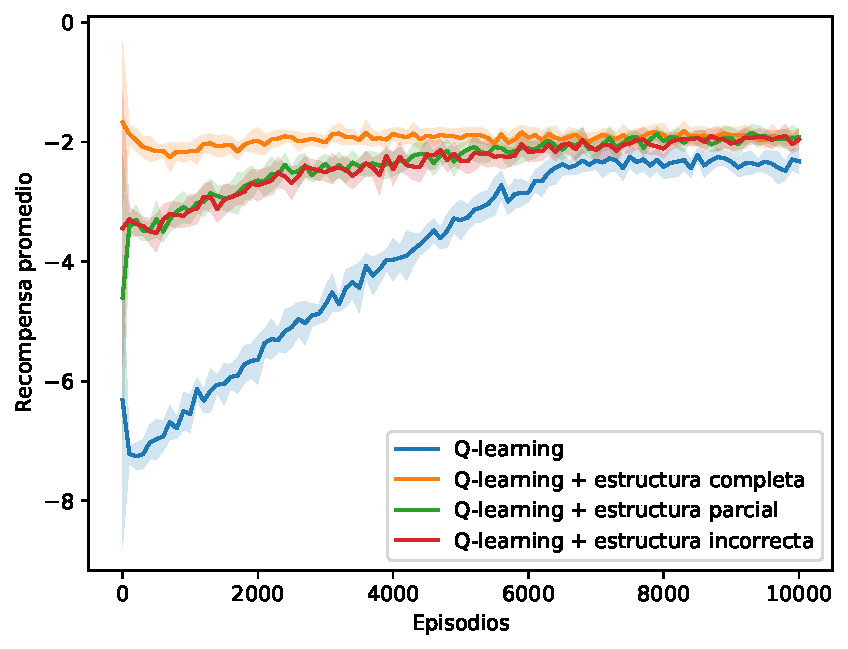
\includegraphics[width=.32\linewidth]{Chapter5/Figs/exp1/low/comparison_10_5_one_to_one_10000_deterministic_eps_partition_50.pdf}&
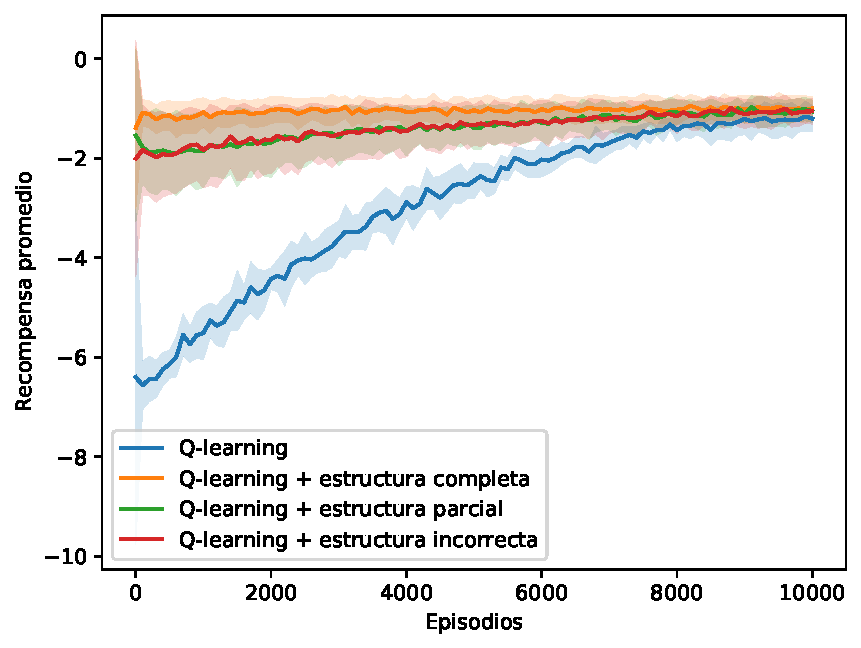
\includegraphics[width=.32\linewidth]{Chapter5/Figs/exp1/low/comparison_10_5_one_to_many_10000_deterministic_eps_partition_50.pdf}&
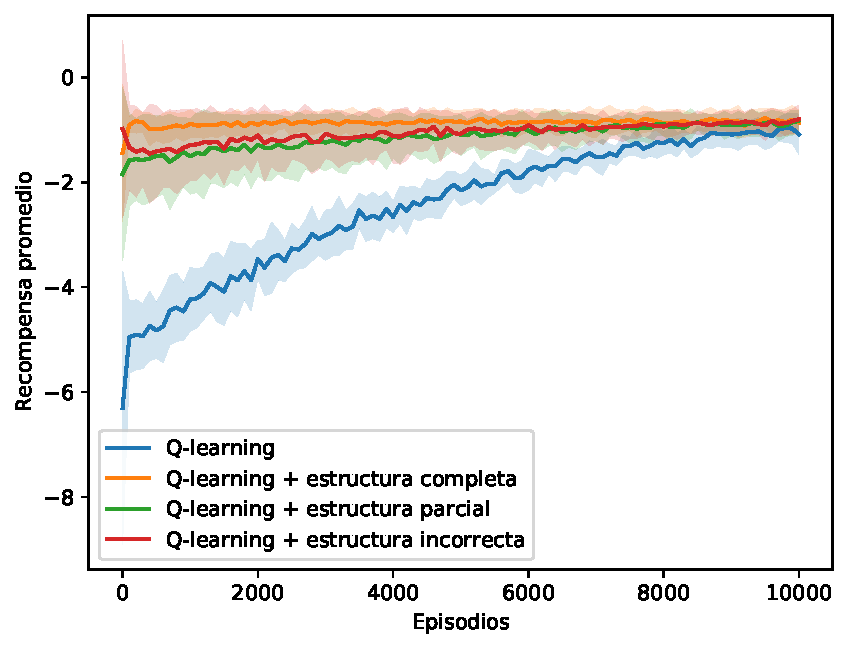
\includegraphics[width=.32\linewidth]{Chapter5/Figs/exp1/low/comparison_10_5_many_to_one_10000_deterministic_eps_partition_50.pdf}
\\
\rowname{$N=7$}&
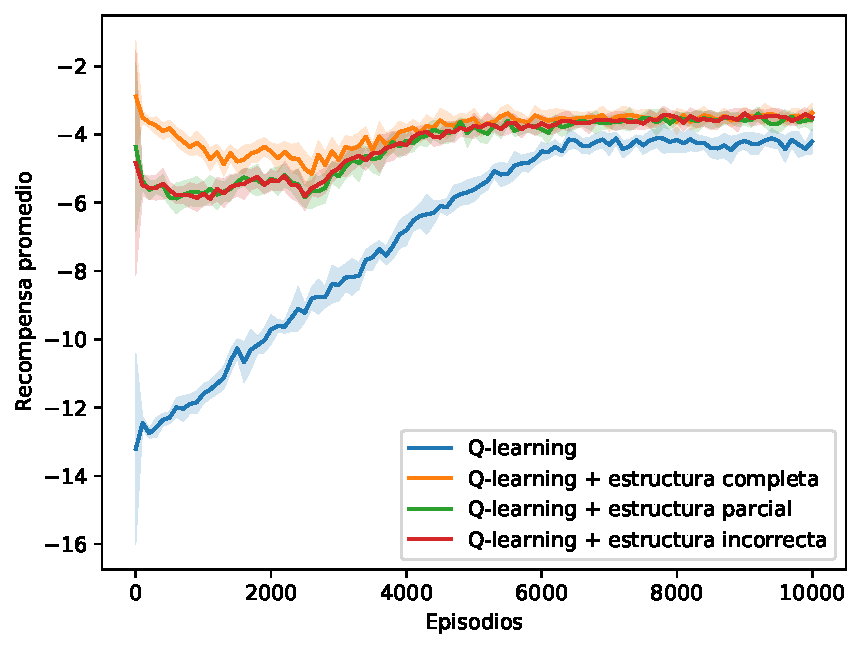
\includegraphics[width=.32\linewidth]{Chapter5/Figs/exp1/low/comparison_10_7_one_to_one_10000_deterministic_eps_partition_50.pdf}&
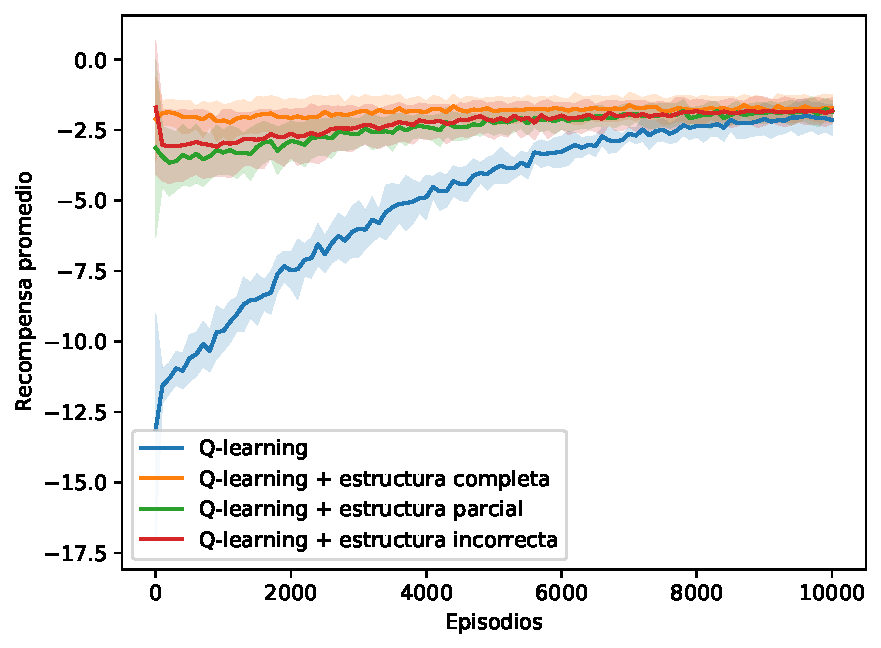
\includegraphics[width=.32\linewidth]{Chapter5/Figs/exp1/low/comparison_10_7_one_to_many_10000_deterministic_eps_partition_50.pdf}&
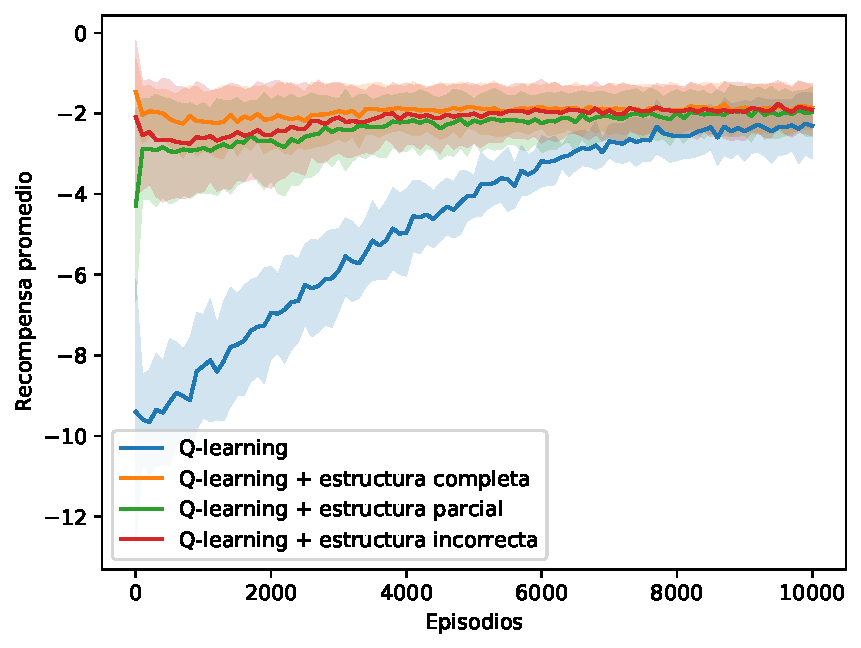
\includegraphics[width=.32\linewidth]{Chapter5/Figs/exp1/low/comparison_10_7_many_to_one_10000_deterministic_eps_partition_50.pdf}\\
\rowname{$N = 9$}&
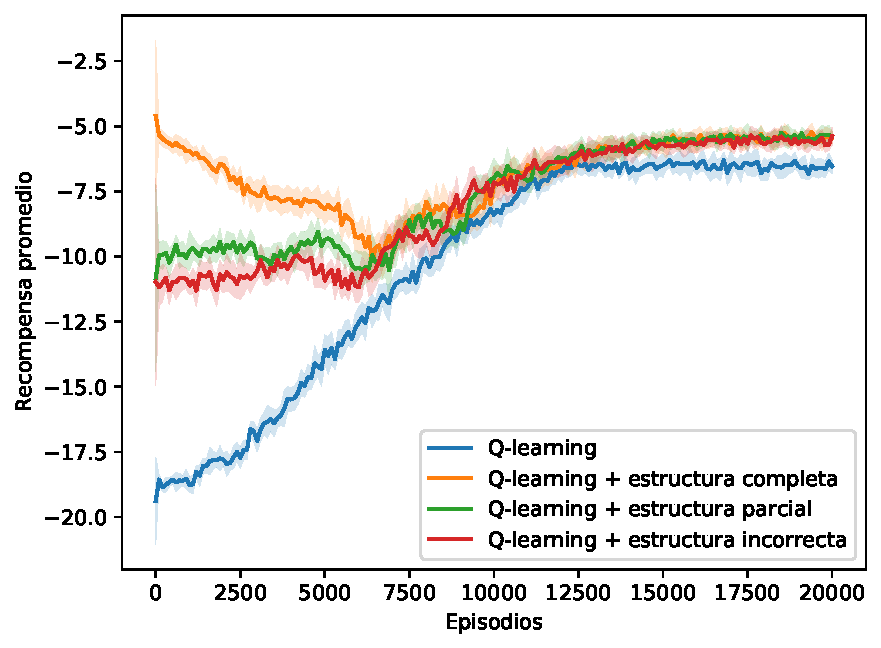
\includegraphics[width=.32\linewidth]{Chapter5/Figs/exp1/low/comparison_10_9_one_to_one_20000_deterministic_eps_partition_50.pdf}&
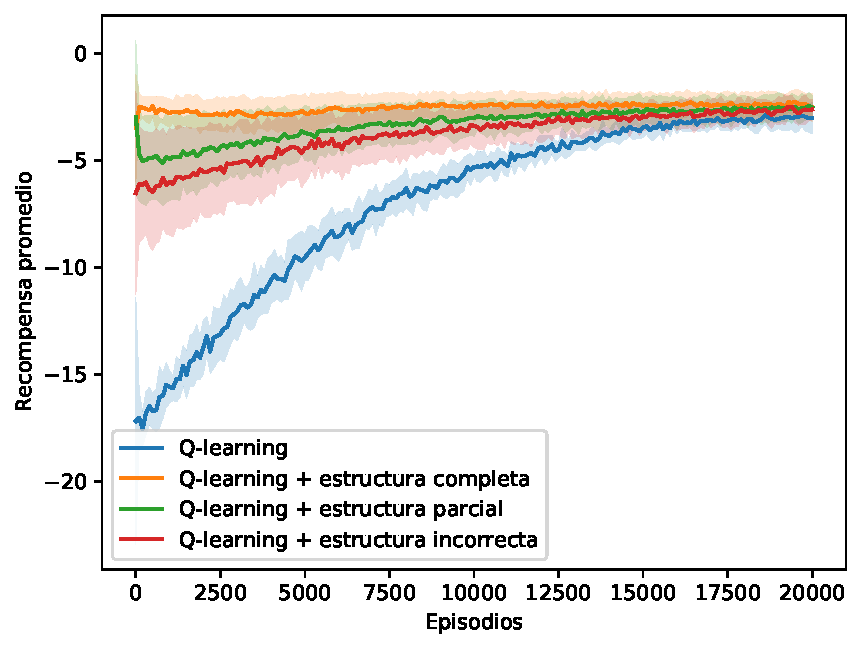
\includegraphics[width=.32\linewidth]{Chapter5/Figs/exp1/low/comparison_10_9_one_to_many_20000_deterministic_eps_partition_50.pdf}&
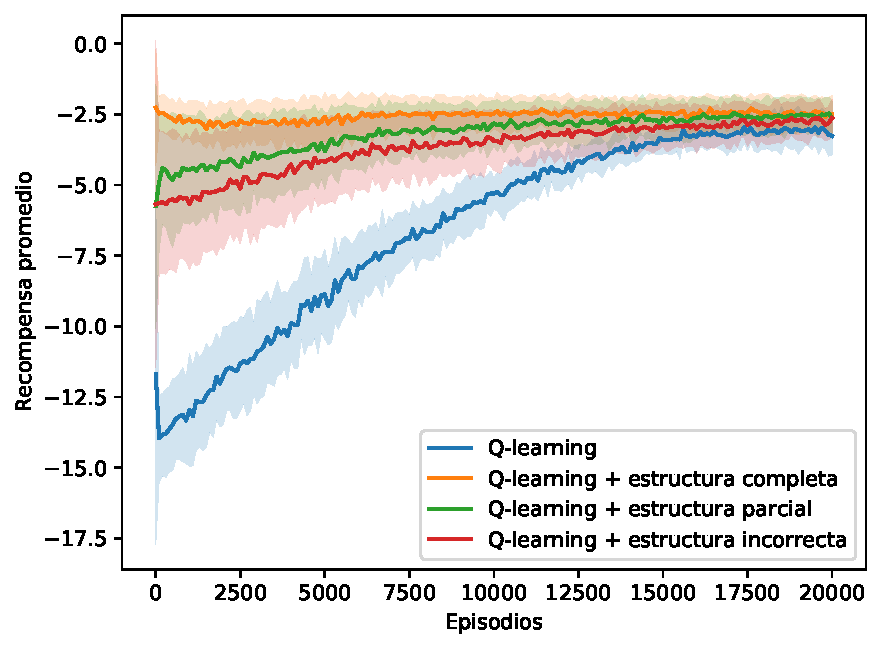
\includegraphics[width=.32\linewidth]{Chapter5/Figs/exp1/low/comparison_10_9_many_to_one_20000_deterministic_eps_partition_50.pdf}

\end{tabular}
\caption{Comparación del desempeño para los 4 algoritmos con un nivel de alteración $p_{mod} = 25 \%$ en un ambiente determinista. Las gráficas muestran la medida $average$ y la desviación estándar (región sombreada) para 10 experimentos.}
\label{fig:low-mod-det}
\end{figure}

\begin{figure}
\settoheight{\tempdima}{\includegraphics[width=.32\linewidth]{example-image-a}}%
\centering\begin{tabular}{@{}c@{ }c@{ }c@{ }c@{}}
&\textbf{Uno-a-uno} & \textbf{Causa común} & \textbf{Efecto común} \\
\rowname{$N = 5$}&
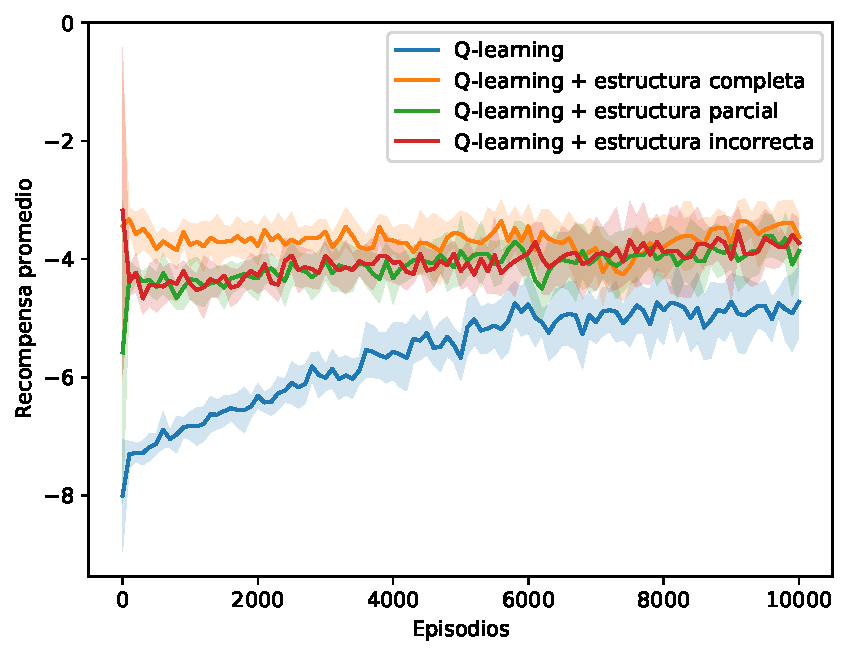
\includegraphics[width=.32\linewidth]{Chapter5/Figs/exp1/low/comparison_10_5_one_to_one_10000_stochastic_eps_partition_50.pdf}&
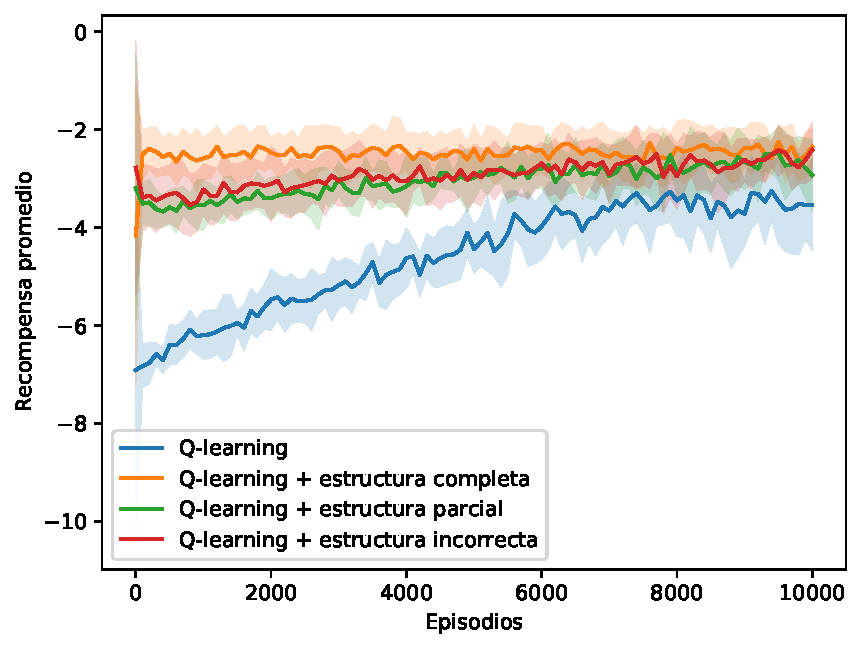
\includegraphics[width=.32\linewidth]{Chapter5/Figs/exp1/low/comparison_10_5_one_to_many_10000_stochastic_eps_partition_50.pdf}&
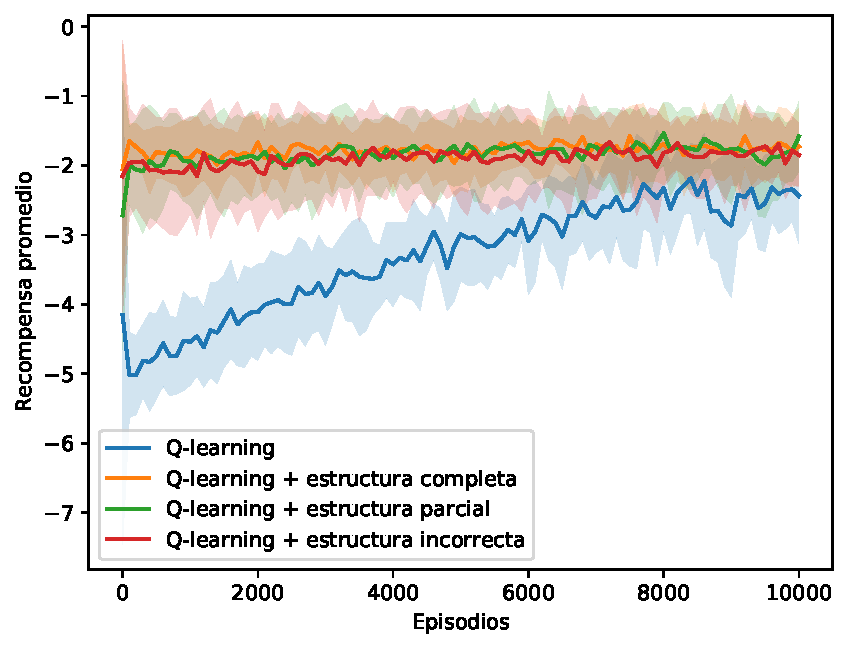
\includegraphics[width=.32\linewidth]{Chapter5/Figs/exp1/low/comparison_10_5_many_to_one_10000_stochastic_eps_partition_50.pdf}\\
\rowname{$N=7$}&
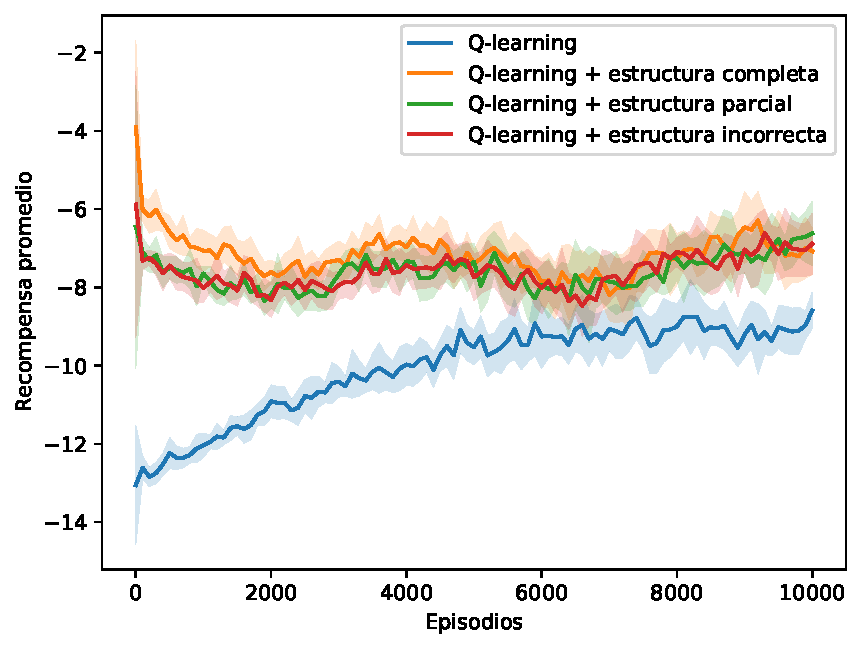
\includegraphics[width=.32\linewidth]{Chapter5/Figs/exp1/low/comparison_10_7_one_to_one_10000_stochastic_eps_partition_50.pdf}&
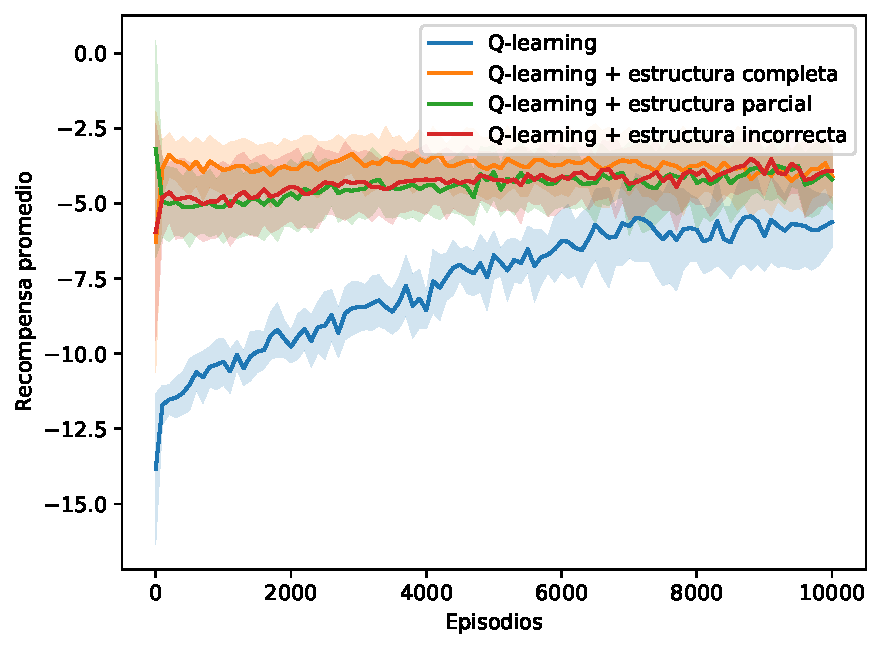
\includegraphics[width=.32\linewidth]{Chapter5/Figs/exp1/low/comparison_10_7_one_to_many_10000_stochastic_eps_partition_50.pdf}&
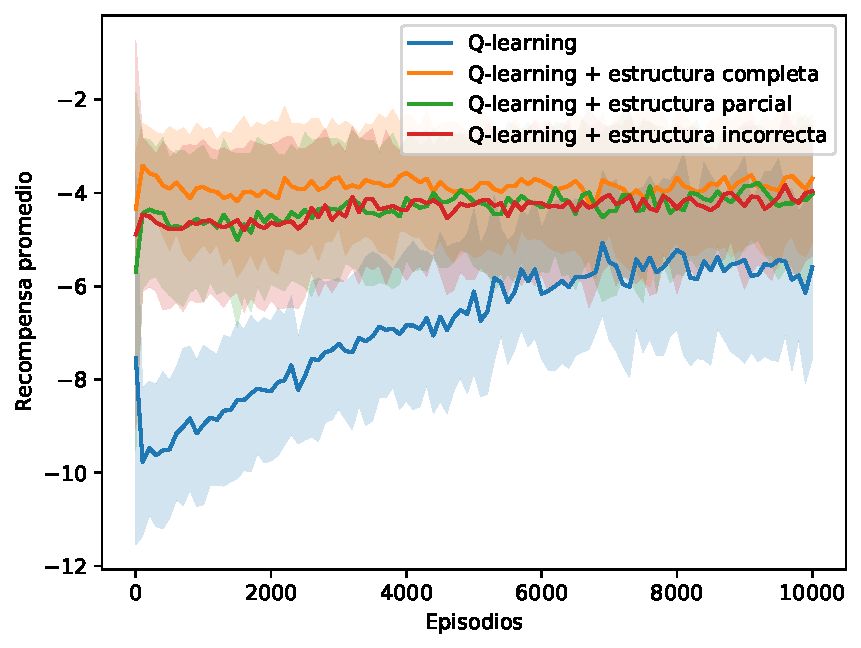
\includegraphics[width=.32\linewidth]{Chapter5/Figs/exp1/low/comparison_10_7_many_to_one_10000_stochastic_eps_partition_50.pdf}\\
\rowname{$N = 9$}&
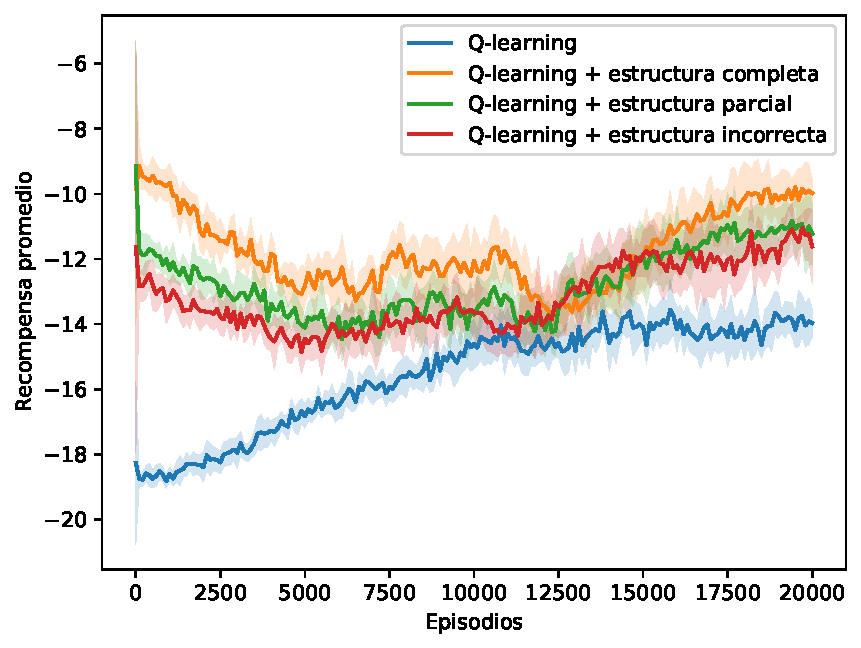
\includegraphics[width=.32\linewidth]{Chapter5/Figs/exp1/low/comparison_10_9_one_to_one_20000_stochastic_eps_partition_50.pdf}&
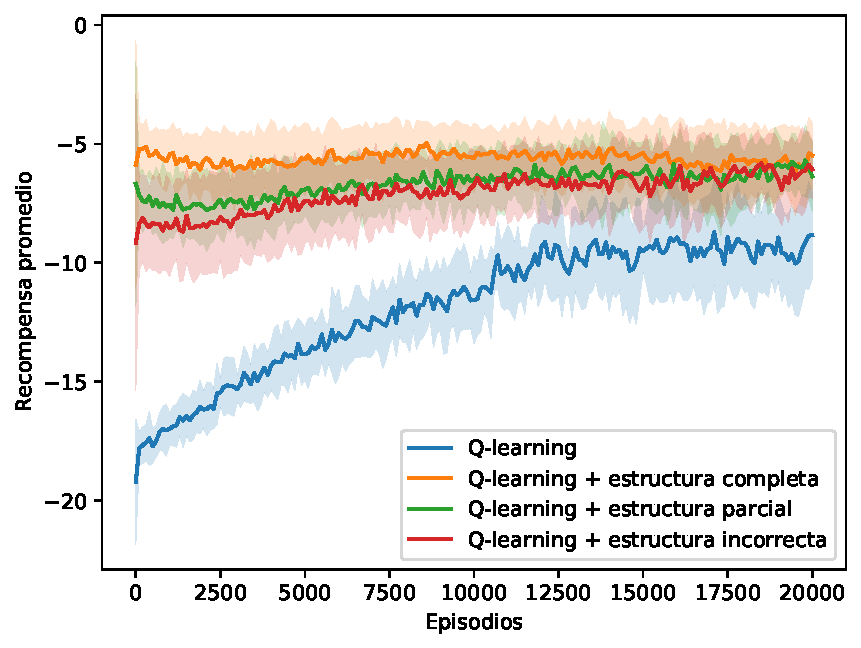
\includegraphics[width=.32\linewidth]{Chapter5/Figs/exp1/low/comparison_10_9_one_to_many_20000_stochastic_eps_partition_50.pdf}&
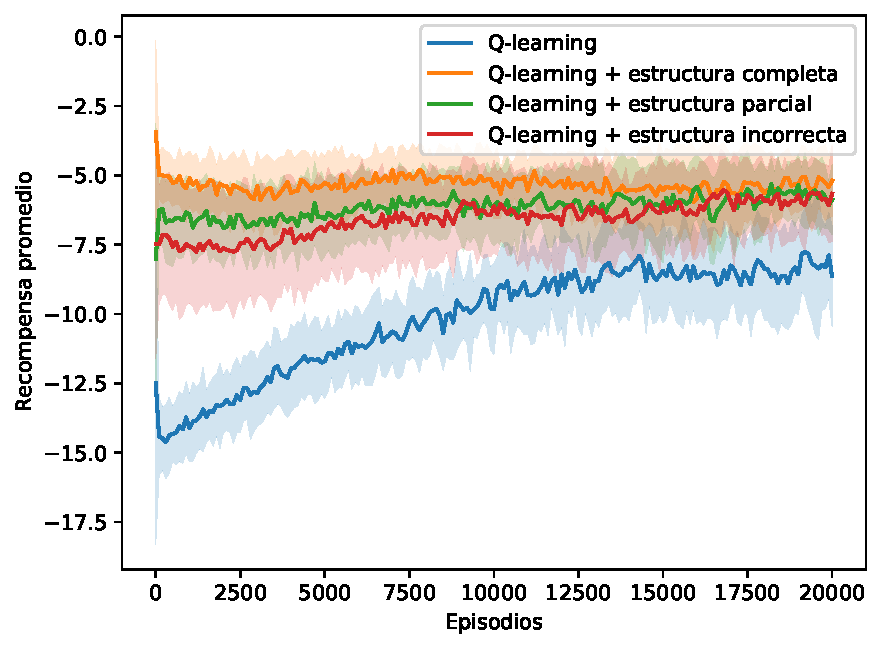
\includegraphics[width=.32\linewidth]{Chapter5/Figs/exp1/low/comparison_10_9_many_to_one_20000_stochastic_eps_partition_50.pdf}

\end{tabular}
\caption{Comparación del desempeño para los 4 algoritmos con un nivel de alteración $p_{mod} = 25 \%$ en un ambiente estocástico. Las gráficas muestran la medida $average$ y la desviación estándar (región sombreada) para 10 experimentos.}
\label{fig:low-mod-sto}
\end{figure}


\begin{figure}
\settoheight{\tempdima}{\includegraphics[width=.32\linewidth]{example-image-a}}%
\centering\begin{tabular}{@{}c@{ }c@{ }c@{ }c@{}}
&\textbf{Uno-a-uno} & \textbf{Causa común} & \textbf{Efecto común} \\
\rowname{$N = 5$}&
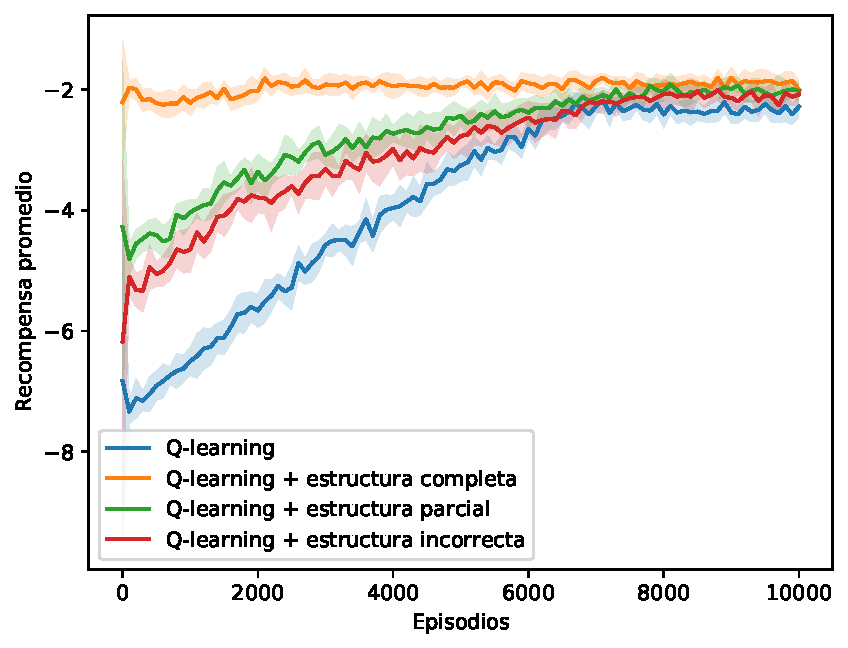
\includegraphics[width=.32\linewidth]{Chapter5/Figs/exp1/medium/comparison_10_5_one_to_one_10000_deterministic_eps_partition_50.pdf}&
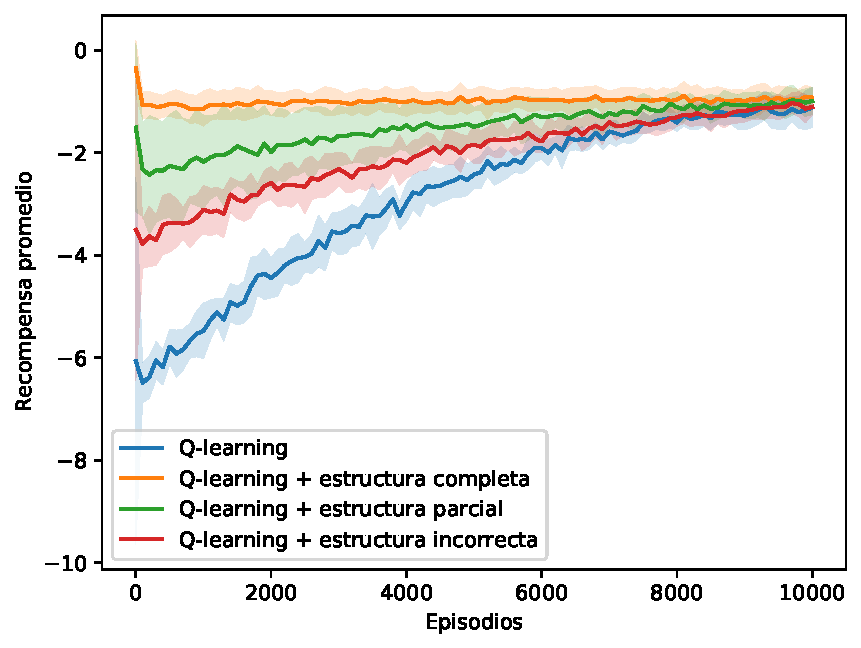
\includegraphics[width=.32\linewidth]{Chapter5/Figs/exp1/medium/comparison_10_5_one_to_many_10000_deterministic_eps_partition_50.pdf}&
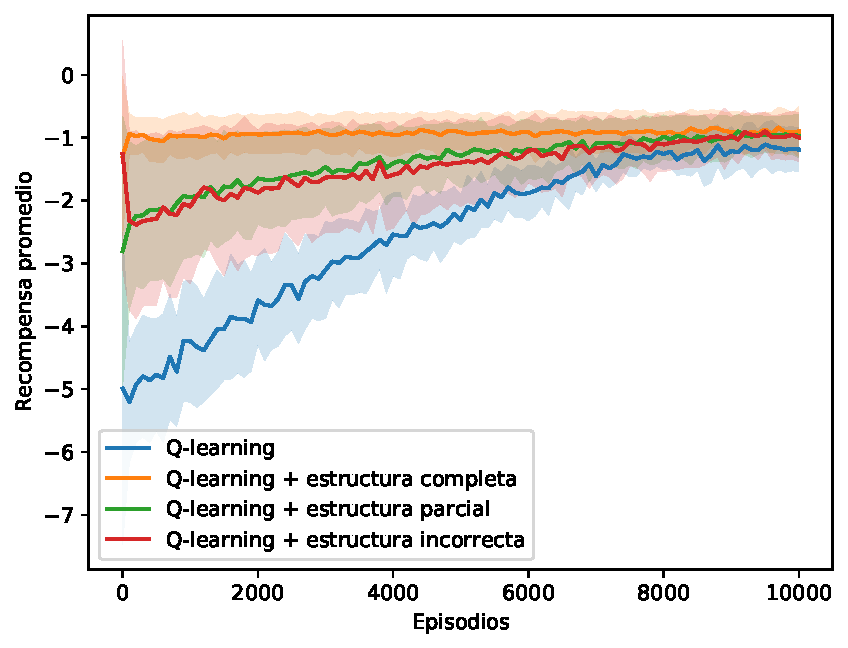
\includegraphics[width=.32\linewidth]{Chapter5/Figs/exp1/medium/comparison_10_5_many_to_one_10000_deterministic_eps_partition_50.pdf}\\
\rowname{$N=7$}&
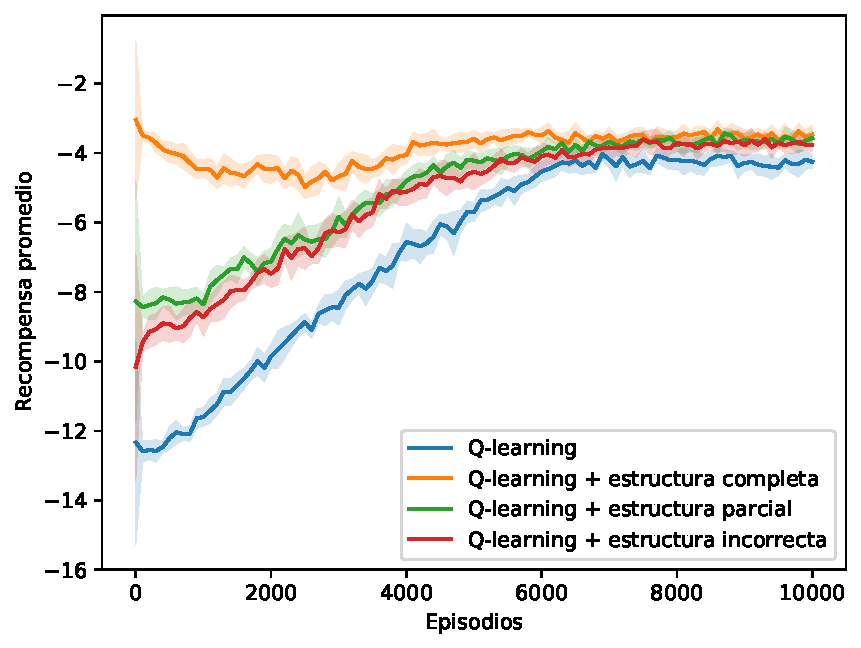
\includegraphics[width=.32\linewidth]{Chapter5/Figs/exp1/medium/comparison_10_7_one_to_one_10000_deterministic_eps_partition_50.pdf}&
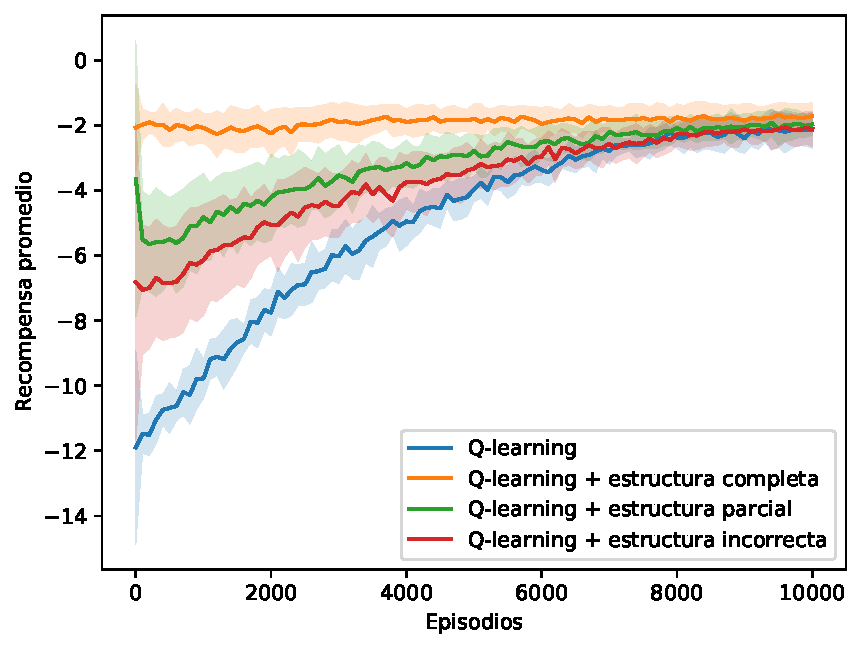
\includegraphics[width=.32\linewidth]{Chapter5/Figs/exp1/medium/comparison_10_7_one_to_many_10000_deterministic_eps_partition_50.pdf}&
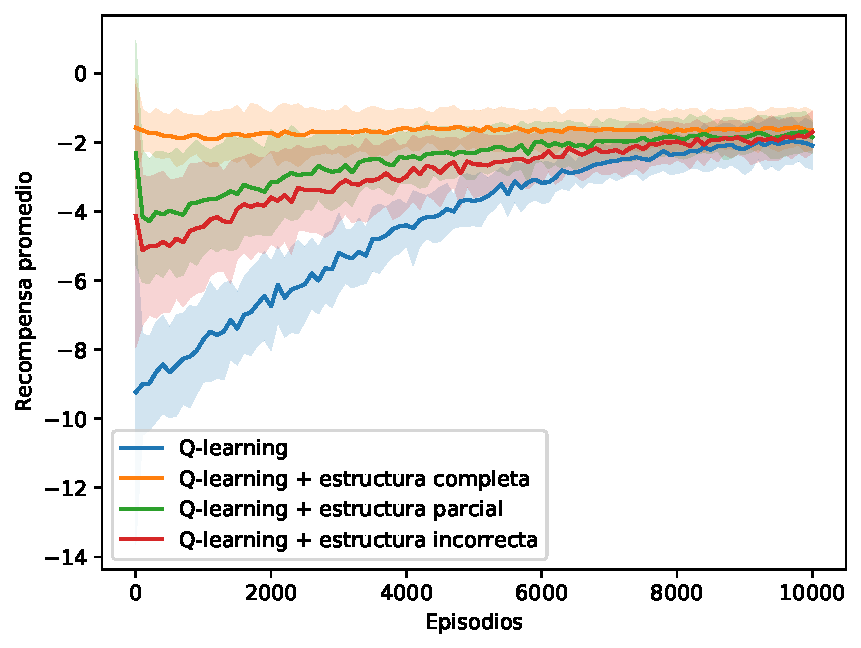
\includegraphics[width=.32\linewidth]{Chapter5/Figs/exp1/medium/comparison_10_7_many_to_one_10000_deterministic_eps_partition_50.pdf}\\
\rowname{$N = 9$}&
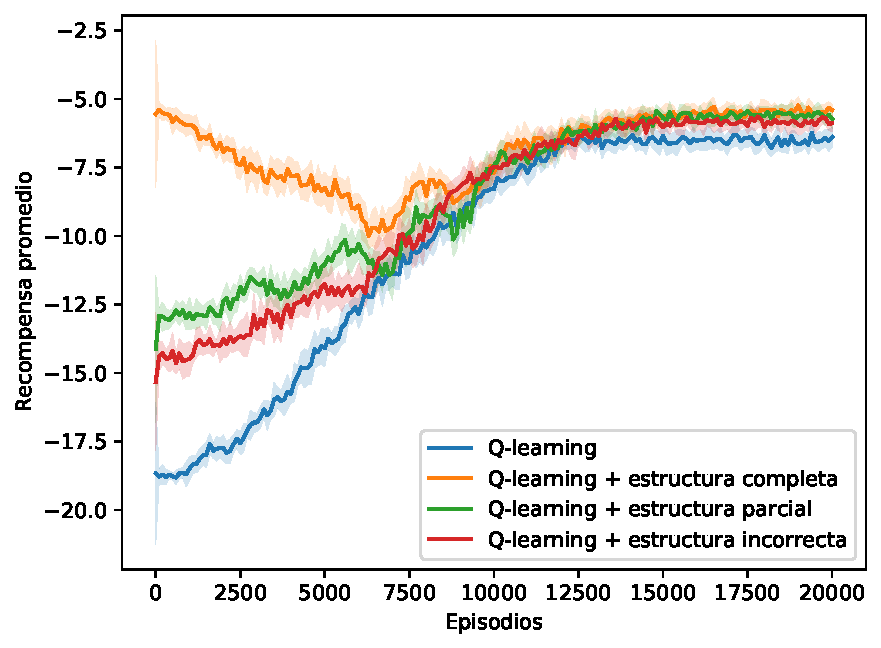
\includegraphics[width=.32\linewidth]{Chapter5/Figs/exp1/medium/comparison_10_9_one_to_one_20000_deterministic_eps_partition_50.pdf}&
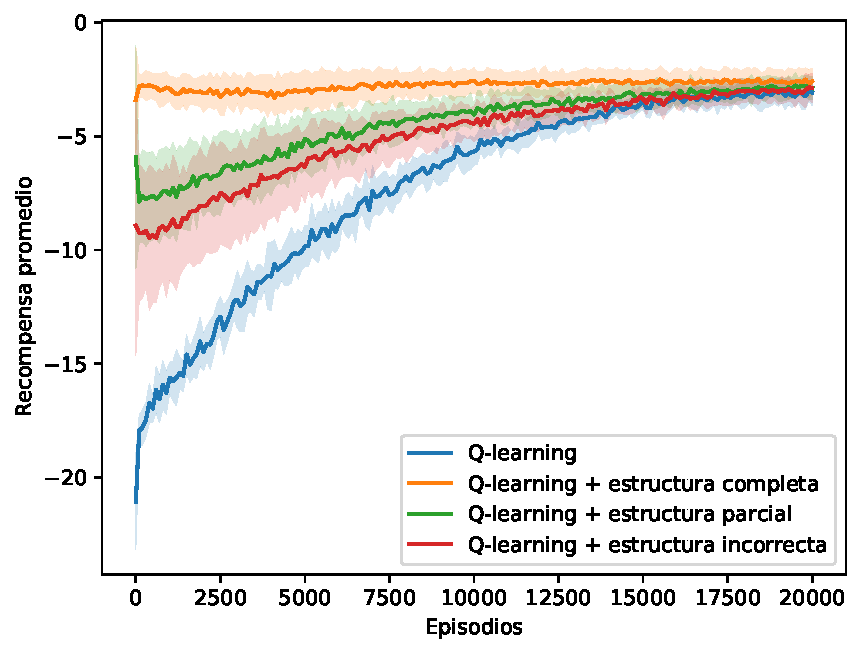
\includegraphics[width=.32\linewidth]{Chapter5/Figs/exp1/medium/comparison_10_9_one_to_many_20000_deterministic_eps_partition_50.pdf}&
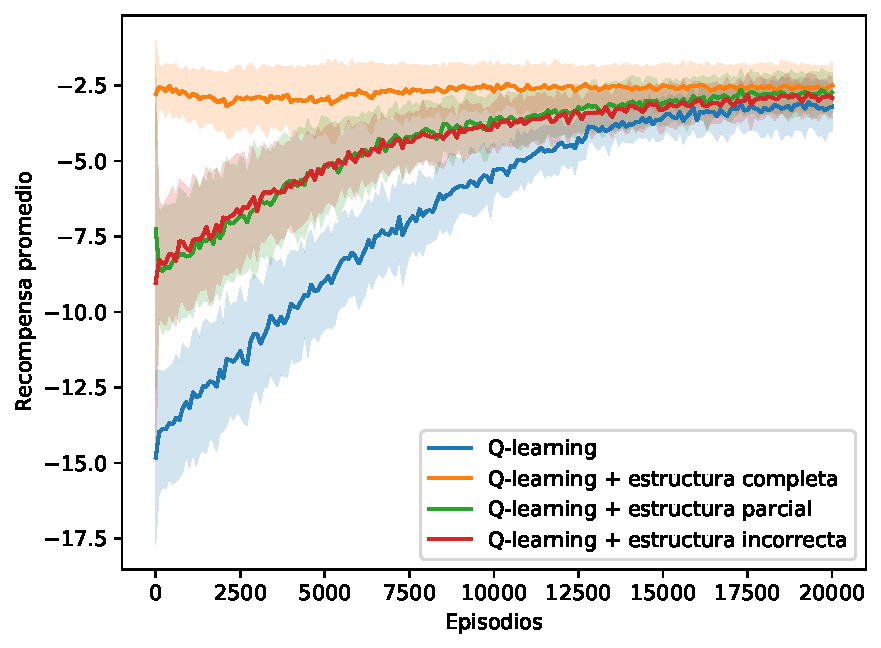
\includegraphics[width=.32\linewidth]{Chapter5/Figs/exp1/medium/comparison_10_9_many_to_one_20000_deterministic_eps_partition_50.pdf}

\end{tabular}
\caption{Comparación del desempeño para los 4 algoritmos con un nivel de alteración $p_{mod} = 50 \%$ en un ambiente determinista. Las gráficas muestran la medida $average$ y la desviación estándar (región sombreada) para 10 experimentos.}
\label{fig:med-mod-det}
\end{figure}

% \begin{figure}
% \settoheight{\tempdima}{\includegraphics[width=.32\linewidth]{example-image-a}}%
% \centering\begin{tabular}{@{}c@{ }c@{ }c@{ }c@{}}
% &\textbf{Uno-a-uno} & \textbf{Causa común} & \textbf{Efecto común} \\
% \rowname{$N = 5$}&
% \includegraphics[width=.32\linewidth]{example-image-a}&
% \includegraphics[width=.32\linewidth]{example-image-b}&
% \includegraphics[width=.32\linewidth]{example-image-c}\\
% \rowname{$N=7$}&
% \includegraphics[width=.32\linewidth]{example-image-a}&
% \includegraphics[width=.32\linewidth]{example-image-b}&
% \includegraphics[width=.32\linewidth]{example-image-c}\\
% \rowname{$N = 9$}&
% \includegraphics[width=.32\linewidth]{example-image-a}&
% \includegraphics[width=.32\linewidth]{example-image-b}&
% \includegraphics[width=.32\linewidth]{example-image-c}

% \end{tabular}
% \caption{Comparación del desempeño para los 4 algoritmos con un nivel de alteración $p_{mod} = 50 \%$ en un ambiente estocástico. Las gráficas muestran la medida $average$ y la desviación estándar (región sombreada) para 10 experimentos.}
% \label{fig:med-mod-sto}
% \end{figure}


\begin{figure}
\settoheight{\tempdima}{\includegraphics[width=.32\linewidth]{example-image-a}}%
\centering\begin{tabular}{@{}c@{ }c@{ }c@{ }c@{}}
&\textbf{Uno-a-uno} & \textbf{Causa común} & \textbf{Efecto común} \\
\rowname{$N = 5$}&
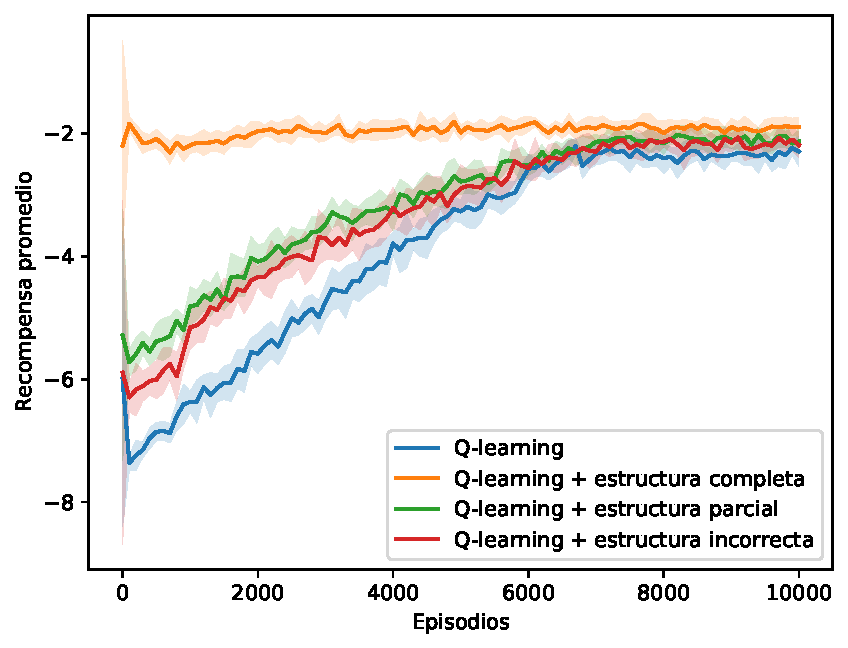
\includegraphics[width=.32\linewidth]{Chapter5/Figs/exp1/high/comparison_10_5_one_to_one_10000_deterministic_eps_partition_50.pdf}&
\includegraphics[width=.32\linewidth]{Chapter5/Figs/exp1/high/comparison_10_5_one_to_many_10000_deterministic_eps_partition_50.pdf}&
\includegraphics[width=.32\linewidth]{Chapter5/Figs/exp1/high/comparison_10_5_many_to_one_10000_deterministic_eps_partition_50.pdf}\\
\rowname{$N=7$}&
\includegraphics[width=.32\linewidth]{Chapter5/Figs/exp1/high/comparison_10_7_one_to_one_10000_deterministic_eps_partition_50.pdf}&
\includegraphics[width=.32\linewidth]{Chapter5/Figs/exp1/high/comparison_10_7_one_to_many_10000_deterministic_eps_partition_50.pdf}&
\includegraphics[width=.32\linewidth]{Chapter5/Figs/exp1/high/comparison_10_7_many_to_one_10000_deterministic_eps_partition_50.pdf}\\
\rowname{$N = 9$}&
\includegraphics[width=.32\linewidth]{Chapter5/Figs/exp1/high/comparison_10_9_one_to_one_20000_deterministic_eps_partition_50.pdf}&
\includegraphics[width=.32\linewidth]{Chapter5/Figs/exp1/high/comparison_10_9_one_to_many_20000_deterministic_eps_partition_50.pdf}&
\includegraphics[width=.32\linewidth]{Chapter5/Figs/exp1/high/comparison_10_9_many_to_one_20000_deterministic_eps_partition_50.pdf}

\end{tabular}
\caption{Comparación del desempeño para los 4 algoritmos con un nivel de alteración $p_{mod} = 75 \%$ en un ambiente determinista. Las gráficas muestran la medida $average$ y la desviación estándar (región sombreada) para 10 experimentos.}
\label{fig:high-mod-det}
\end{figure}

% \begin{figure}
% \settoheight{\tempdima}{\includegraphics[width=.32\linewidth]{example-image-a}}%
% \centering\begin{tabular}{@{}c@{ }c@{ }c@{ }c@{}}
% &\textbf{Uno-a-uno} & \textbf{Causa común} & \textbf{Efecto común} \\
% \rowname{$N = 5$}&
% \includegraphics[width=.32\linewidth]{example-image-a}&
% \includegraphics[width=.32\linewidth]{example-image-b}&
% \includegraphics[width=.32\linewidth]{example-image-c}\\
% \rowname{$N=7$}&
% \includegraphics[width=.32\linewidth]{example-image-a}&
% \includegraphics[width=.32\linewidth]{example-image-b}&
% \includegraphics[width=.32\linewidth]{example-image-c}\\
% \rowname{$N = 9$}&
% \includegraphics[width=.32\linewidth]{example-image-a}&
% \includegraphics[width=.32\linewidth]{example-image-b}&
% \includegraphics[width=.32\linewidth]{example-image-c}

% \end{tabular}
% \caption{Comparación del desempeño para los 4 algoritmos con un nivel de alteración $p_{mod} = 75 \%$ en un ambiente estocástico. Las gráficas muestran la medida $average$ y la desviación estándar (región sombreada) para 10 experimentos.}
% \label{fig:high-mod-sto}
% \end{figure}


\newpage

\subsection{Explotar o seguir explorando}\label{subsection:exp-epsilon}


\begin{itemize}
    \item El espacio de estados es discreto, es decir, el agente puede
    obtener las variables $\mathcal{X}$ directamente del ambiente.
    \item Para obtener a los
    grafos $\mathcal{D'}$ y $\mathcal{D''}$,
    el porcentaje de nivel de cambio  es $p_{mod} = 25 \%$. Esto significa que no se altera demasiado el grafo causal original para
    generar los grafos incompletos e incorrectos.
    \item Se controla qué tan rápido se desea alcanzar $\epsilon_{\min}$ variando el parámetro $\delta$. Si se divide al entrenamiento en cuartos,  entonces los valores de $\delta$ corresponden a en qué cuarto se alcanza el mínimo valor para $\epsilon$.
    \begin{itemize}
        \item Alcanzar $\epsilon_{\min}$ en el primer cuarto del entrenamiento, $\delta = 0.25$.
        \item Alcanzar $\epsilon_{\min}$ a medio aprendizaje, $\delta = 0.50$.
        \item Alcanzar $\epsilon_{\min}$ en el tercer cuarto del entrenamiento, $\delta = 0.75$.
    \end{itemize}
    \item Se examina sobre los tres tipos de estructuras posibles: uno-a-uno, 
    causa común y efecto común. 
    \item Se prueba sobre un mundo determinista.
\end{itemize}

\subsubsection{Objetivo}

Determinar si reducir o aumentar las consultas al grafo causal a lo largo del aprendizaje afecta el desempeño
de los algoritmos.

\subsubsection{Hipótesis}

La información del grafo causal no afecta negativamente 
el aprendizaje de la función de valor $Q$. Por lo tanto, incluso si se disminuyen las consultas al modelo de manera temprana en el entrenamiento, la información provista habrá
ayudado al aprendizaje de la función.

\subsubsection{Resultados}

En las Figuras \ref{fig:low-epsilon-det} y \ref{fig:high-epsilon-det} se puede ver que los algoritmos que utilizan conocimiento del grafo inician con una recompensa mayor y se estabilizan más rápido que el algoritmo Q-learning
sin información adicional en ambientes con transiciones deterministas. 
De acuerdo con los resultados parece que 
entre mayor sea $\delta$ más tarda en estabilizarse
el algoritmo de aprendizaje sin información que lo auxilie. Esto es de esperarse, ya que se sigue explorando durante más tiempo. Sin embargo,
también se puede notar que estimula a dejar
la exploración de manera temprana, no implica que después
de dejarla, el algoritmo converge inmediatamente. Por otro lado, 
la recompensa, en los algoritmos que se guían por el grafo, se desestabiliza
el intervalo en el que se encuentra la transición a dejar de dar peso a 
la exploración. Pero, una vez fuera de esa ``zona de transición'' los
algoritmos se recuperan y tienden a estar por encima del algoritmo sin datos 
extra.


\begin{figure}
\settoheight{\tempdima}{\includegraphics[width=.32\linewidth]{example-image-a}}%
\centering\begin{tabular}{@{}c@{ }c@{ }c@{ }c@{}}
&\textbf{Uno-a-uno} & \textbf{Causa común} & \textbf{Efecto común} \\
\rowname{$N = 5$}&
\includegraphics[width=.32\linewidth]{Chapter5/Figs/exp2/low/comparison_10_5_one_to_one_5000_deterministic_eps_partition_25.pdf}&
\includegraphics[width=.32\linewidth]{Chapter5/Figs/exp2/low/comparison_10_5_one_to_many_5000_deterministic_eps_partition_25.pdf}&
\includegraphics[width=.32\linewidth]{Chapter5/Figs/exp2/low/comparison_10_5_many_to_one_5000_deterministic_eps_partition_25.pdf}\\
\rowname{$N=7$}&
\includegraphics[width=.32\linewidth]{Chapter5/Figs/exp2/low/comparison_10_7_one_to_one_5000_deterministic_eps_partition_25.pdf}&
\includegraphics[width=.32\linewidth]{Chapter5/Figs/exp2/low/comparison_10_7_one_to_many_5000_deterministic_eps_partition_25.pdf}&
\includegraphics[width=.32\linewidth]{Chapter5/Figs/exp2/low/comparison_10_7_many_to_one_5000_deterministic_eps_partition_25.pdf}\\
\rowname{$N = 9$}&
\includegraphics[width=.32\linewidth]{Chapter5/Figs/exp2/low/comparison_10_9_one_to_one_10000_deterministic_eps_partition_25.pdf}&
\includegraphics[width=.32\linewidth]{Chapter5/Figs/exp2/low/comparison_10_9_one_to_many_10000_deterministic_eps_partition_25.pdf}&
\includegraphics[width=.32\linewidth]{Chapter5/Figs/exp2/low/comparison_10_9_many_to_one_10000_deterministic_eps_partition_25.pdf}
\end{tabular}
\caption{Comparación del desempeño para los 4 algoritmos con un nivel de alteración $p_{mod} = 25 \%$  y $\delta = 0.25$ en un ambiente determinista. Las gráficas muestran la medida $average$ y la desviación estándar (región sombreada) para 10 experimentos.}
\label{fig:low-epsilon-det}
\end{figure}

% \begin{figure}
% \settoheight{\tempdima}{\includegraphics[width=.32\linewidth]{example-image-a}}%
% \centering\begin{tabular}{@{}c@{ }c@{ }c@{ }c@{}}
% &\textbf{Uno-a-uno} & \textbf{Causa común} & \textbf{Efecto común} \\
% \rowname{$N = 5$}&
% \includegraphics[width=.32\linewidth]{example-image-a}&
% \includegraphics[width=.32\linewidth]{example-image-b}&
% \includegraphics[width=.32\linewidth]{example-image-c}\\
% \rowname{$N=7$}&
% \includegraphics[width=.32\linewidth]{example-image-a}&
% \includegraphics[width=.32\linewidth]{example-image-b}&
% \includegraphics[width=.32\linewidth]{example-image-c}\\
% \rowname{$N = 9$}&
% \includegraphics[width=.32\linewidth]{example-image-a}&
% \includegraphics[width=.32\linewidth]{example-image-b}&
% \includegraphics[width=.32\linewidth]{example-image-c}

% \end{tabular}
% \caption{Comparación del desempeño para los 4 algoritmos con un nivel de alteración $p_{mod} = 75 \%$ en un ambiente estocástico. Las gráficas muestran la medida $average$ y la desviación estándar (región sombreada) para 10 experimentos.}
% \label{fig:low-epsilon-sto}
% \end{figure}

\begin{figure}
\settoheight{\tempdima}{\includegraphics[width=.32\linewidth]{example-image-a}}%
\centering\begin{tabular}{@{}c@{ }c@{ }c@{ }c@{}}
&\textbf{Uno-a-uno} & \textbf{Causa común} & \textbf{Efecto común} \\
\rowname{$N = 5$}&
\includegraphics[width=.32\linewidth]{example-image-a}&
\includegraphics[width=.32\linewidth]{Chapter5/Figs/exp2/high/comparison_10_5_one_to_many_5000_deterministic_eps_partition_75.pdf}&
\includegraphics[width=.32\linewidth]{Chapter5/Figs/exp2/high/comparison_10_5_many_to_one_5000_deterministic_eps_partition_75.pdf}\\
\rowname{$N=7$}&
\includegraphics[width=.32\linewidth]{example-image-a}&
\includegraphics[width=.32\linewidth]{Chapter5/Figs/exp2/high/comparison_10_7_one_to_many_5000_deterministic_eps_partition_75.pdf}&
\includegraphics[width=.32\linewidth]{Chapter5/Figs/exp2/high/comparison_10_7_many_to_one_5000_deterministic_eps_partition_75.pdf}\\
\rowname{$N = 9$}&
\includegraphics[width=.32\linewidth]{example-image-a}&
\includegraphics[width=.32\linewidth]{Chapter5/Figs/exp2/high/comparison_10_9_one_to_many_10000_deterministic_eps_partition_75.pdf}&
\includegraphics[width=.32\linewidth]{Chapter5/Figs/exp2/high/comparison_10_9_many_to_one_10000_deterministic_eps_partition_75.pdf}
\end{tabular}
\caption{Comparación del desempeño para los 4 algoritmos con un nivel de alteración $p_{mod} = 25 \%$ y $\delta = 0.75$ en un ambiente determinista. Las gráficas muestran la medida $average$ y la desviación estándar (región sombreada) para 10 experimentos.}
\label{fig:high-epsilon-det}
\end{figure}

% \begin{figure}
% \settoheight{\tempdima}{\includegraphics[width=.32\linewidth]{example-image-a}}%
% \centering\begin{tabular}{@{}c@{ }c@{ }c@{ }c@{}}
% &\textbf{Uno-a-uno} & \textbf{Causa común} & \textbf{Efecto común} \\
% \rowname{$N = 5$}&
% \includegraphics[width=.32\linewidth]{example-image-a}&
% \includegraphics[width=.32\linewidth]{example-image-b}&
% \includegraphics[width=.32\linewidth]{example-image-c}\\
% \rowname{$N=7$}&
% \includegraphics[width=.32\linewidth]{example-image-a}&
% \includegraphics[width=.32\linewidth]{example-image-b}&
% \includegraphics[width=.32\linewidth]{example-image-c}\\
% \rowname{$N = 9$}&
% \includegraphics[width=.32\linewidth]{example-image-a}&
% \includegraphics[width=.32\linewidth]{example-image-b}&
% \includegraphics[width=.32\linewidth]{example-image-c}

% \end{tabular}
% \caption{Comparación del desempeño para los 4 algoritmos con un nivel de alteración $p_{mod} = 75 \%$ en un ambiente estocástico. Las gráficas muestran la medida $average$ y la desviación estándar (región sombreada) para 10 experimentos.}
% \label{fig:med-epsilon-sto}
% \end{figure}

% \begin{figure}
% \settoheight{\tempdima}{\includegraphics[width=.32\linewidth]{example-image-a}}%
% \centering\begin{tabular}{@{}c@{ }c@{ }c@{ }c@{}}
% &\textbf{Uno-a-uno} & \textbf{Causa común} & \textbf{Efecto común} \\
% \rowname{$N = 5$}&
% \includegraphics[width=.32\linewidth]{example-image-a}&
% \includegraphics[width=.32\linewidth]{example-image-b}&
% \includegraphics[width=.32\linewidth]{example-image-c}\\
% \rowname{$N=7$}&
% \includegraphics[width=.32\linewidth]{example-image-a}&
% \includegraphics[width=.32\linewidth]{example-image-b}&
% \includegraphics[width=.32\linewidth]{example-image-c}\\
% \rowname{$N = 9$}&
% \includegraphics[width=.32\linewidth]{example-image-a}&
% \includegraphics[width=.32\linewidth]{example-image-b}&
% \includegraphics[width=.32\linewidth]{example-image-c}

% \end{tabular}
% \caption{Comparación del desempeño para los 4 algoritmos con un nivel de alteración $p_{mod} = 75 \%$ en un ambiente estocástico. Las gráficas muestran la medida $average$ y la desviación estándar (región sombreada) para 10 experimentos.}
% \label{fig:high-epsilon-sto}
% \end{figure}

\newpage

\subsection{Utilizando observaciones visuales del ambiente}

\subsubsection{Configuración experimental}

\begin{itemize}
    \item Los elementos del espacio de estados $\mathcal{S}$, son continuos.
    Las observaciones son imágenes de $84\times 84$ pixeles en un espacio de color RGB, obtenidas desde una vista cenital del ambiente.
    
    \begin{figure}[H]
        \centering
        \includegraphics[scale=0.2]{Chapter5/Figs/obs_example.png}
        \caption{Ejemplo de una posible observación del agente.}
        \label{fig:obs-example-lights}
    \end{figure}
    \item Para mapear las imágenes al espacio de estados de alto nivel $\mathcal{X}$, la función $\phi$ es un clasificador multi etiqueta
    parametrizado por una red neuronal convolucional \cite{Goodfellow-et-al-2016} (CNN por sus siglas en inglés). La arquitectura de la red, de manera visual, se presenta en la Figura \ref{fig:cnn-classifier}. Al agente se le brinda el clasificador ya entrenado.
    La salida de la red son procesadores $p_i$ que
    representan la probabilidad de que la variable $x_i$ tome el valor 1, donde
    $i \in \{1, \dots, l\}$. Por simplicidad se utiliza un solo
    clasificador para los distintos experimentos. Por lo tanto, $l = 9$ y
    para los casos donde $N < 9$ entonces se suponen las variables mayores
    a $N$ como apagadas. 
    \item Las transiciones entre estados son deterministas.
    \item El valor de parámetro de alteración del grafo causal correcto es
    $p_{mod} = 25$.
    \item La tasa de decremento de $\epsilon$ está controlada por el factor $\delta = 0.75$.
    \item Dado que las observaciones son imágenes, se utiliza la versión 
    del algoritmo Q-learning para estados continuos DQN. La arquitectura e hiperparámetros de entrenamiento son los mismos que los del artículo original del método DQN 
    \cite{mnih2015human}. 
    
\begin{figure}
    \centering
    \includegraphics[scale=0.8]{Chapter5/Figs/multilabel_classifier.pdf}
    \caption{Arquitectura del clasificador multi etiqueta, $\phi$, que
    mapea observaciones visuales a un conjunto de variables
    de alto nivel.}
    \label{fig:cnn-classifier}
\end{figure}
\end{itemize}
\subsubsection{Objetivo}

Determinar si el modelo causal con variables  en otro espacio siguen conservando las propiedades
de ayudar en el aprendizaje como en los casos discretos.

\subsubsection{Hipótesis}

Si se cuenta con información de las observaciones
en un espacio más pequeño, pero donde se codifiquen
los estados en alto nivel, se puede apoyar 
al algoritmo de aprendizaje a alcanzar una recompensa
mayor en menos tiempo.

\subsubsection{Resultados}

De acuerdo con la Figura \ref{fig:dqn-results} los algoritmos que utilizan conocimiento del grafo inician con una recompensa mayor y se estabilizan más rápido que el algoritmo DQN
sin información adicional en ambientes con transiciones deterministas. A pesar de que 
el número de episodios
es menor que en el caso 
discreto, parecen mantenerse los mismo resultados 
que en la configuración de un ambiente con observaciones
discretas.

\begin{figure}
\settoheight{\tempdima}{\includegraphics[width=.32\linewidth]{example-image-a}}%
\centering\begin{tabular}{@{}c@{ }c@{ }c@{ }c@{}}
&\textbf{Uno-a-uno} & \textbf{Causa común} & \textbf{Efecto común} \\
\rowname{$N = 5$}&
\includegraphics[width=.32\linewidth]{Chapter5/Figs/dqn_plots/comparison_dqn_20_5_one_to_one_200_det.png}&
\includegraphics[width=.32\linewidth]{Chapter5/Figs/dqn_plots/comparison_dqn_20_5_one_to_many_200_det.png}&
\includegraphics[width=.32\linewidth]{Chapter5/Figs/dqn_plots/comparison_dqn_20_5_many_to_one_200_det.png}\\
\rowname{$N=7$}&
\includegraphics[width=.32\linewidth]{Chapter5/Figs/dqn_plots/comparison_dqn_20_7_one_to_one_200_det.png}&
\includegraphics[width=.32\linewidth]{Chapter5/Figs/dqn_plots/comparison_dqn_20_7_one_to_many_200_det.png}&
\includegraphics[width=.32\linewidth]{Chapter5/Figs/dqn_plots/comparison_dqn_20_7_many_to_one_200_det.png}\\
\rowname{$N = 9$}&
\includegraphics[width=.32\linewidth]{Chapter5/Figs/dqn_plots/comparison_dqn_20_9_one_to_one_200_det.png}&
\includegraphics[width=.32\linewidth]{Chapter5/Figs/dqn_plots/comparison_dqn_20_9_one_to_many_200_det.png}&
\includegraphics[width=.32\linewidth]{Chapter5/Figs/dqn_plots/comparison_dqn_20_9_many_to_one_200_det.png}

\end{tabular}
\caption{Comparación del desempeño para los 4 algoritmos con $p_{mod} = 25 \%$ y $\delta = 75$ en un ambiente determinista y continuo. Las gráficas muestran la medida $average$ y la desviación estándar (región sombreada) para 10 experimentos.}
\label{fig:dqn-results}
\end{figure}

\newpage
\section{Discusión}

Se presentó una extensión de la política de selección
de acciones durante el entrenamiento de un agente tal que utilice la información de una estructura causal. La intuición de que una exploración
guiada es mejor que una búsqueda a ciegas se cumple de acuerdo 
con los experimentos. De la experimentación, se puede ver que incluso tener muy poca información correcta de la estructura causal $\mathcal{D}$ es mejor que
un método que se basa en una exploración aleatoria. También, reducir el número 
de consultas al grafo y motivar la explotación, no afecta de manera nociva el
aprendizaje de la política.

Puesto que lo presentado es una prueba de concepto, los problemas atacados
son pequeños y relativamente simples. Sin embargo, conducen a la búsqueda
de problemas que puedan ponerse en el contexto de procesos de decisión
con una estructura causal subyacente que se brinde o aprenda previamente.

% \begin{itemize}

%     \item Incluir toda la información necesaria para que el estudio
%     pueda ser repetido.
%     \item El propósito principal del reporte es diseminar los hallazgos o resultados.
%     \item Tus hallazgos deben ser descritos con mucho detalle para que el lector los juzgue.
%     \item Además debe haber suficiente detalle para hacer posible
%     transferir cualquier solución a algún otro lugar.
% \end{itemize}    


% \subsection{Esquemas de comparación}
% \subsubsection{Q-learning}
% \subsubsection{Q-learning con estructura causal completa}
% \subsubsection{Q-learning con estructura causal incompleta}
% \subsubsection{Q-learning con estructura causal incorrecta}
% \subsection{Parámetros y medidas de desempeño}

% \section{Resultados}
% \subsection{Ambiente con estados discretos}
% \subsubsection{Experimento 1 - Cambios en el porcentaje de la completitud de $D$}
% \subsubsection{Experimento 2 - Cambios en la tasa de consulta del modelo $\epsilon$}
% \subsubsection{Experimento 3 - Transferencia de conocimiento}
% \subsection{Ambiente con estados continuos}
% \subsubsection{Experimento 1 - Cambios en el porcentaje de la completitud de $D$}
% \subsubsection{Experimento 2 - Cambios en la tasa de consulta del modelo $\epsilon$}
% \subsubsection{Experimento 3 - Transferencia de conocimiento}

% \subsection{Q-learning}
% \subsection{Q-learning con estructura causal completa}
% \subsection{Q-learning con estructura causal incompleta}
% \subsection{Q-learning con estructura causal incorrecta}


